% Options for packages loaded elsewhere
\PassOptionsToPackage{unicode}{hyperref}
\PassOptionsToPackage{hyphens}{url}
%
\documentclass[
  8pt,
  ignorenonframetext,
]{beamer}
\usepackage{pgfpages}
\setbeamertemplate{caption}[numbered]
\setbeamertemplate{caption label separator}{: }
\setbeamercolor{caption name}{fg=normal text.fg}
\beamertemplatenavigationsymbolsempty
% Prevent slide breaks in the middle of a paragraph
\widowpenalties 1 10000
\raggedbottom
\setbeamertemplate{part page}{
  \centering
  \begin{beamercolorbox}[sep=16pt,center]{part title}
    \usebeamerfont{part title}\insertpart\par
  \end{beamercolorbox}
}
\setbeamertemplate{section page}{
  \centering
  \begin{beamercolorbox}[sep=12pt,center]{part title}
    \usebeamerfont{section title}\insertsection\par
  \end{beamercolorbox}
}
\setbeamertemplate{subsection page}{
  \centering
  \begin{beamercolorbox}[sep=8pt,center]{part title}
    \usebeamerfont{subsection title}\insertsubsection\par
  \end{beamercolorbox}
}
\AtBeginPart{
  \frame{\partpage}
}
\AtBeginSection{
  \ifbibliography
  \else
    \frame{\sectionpage}
  \fi
}
\AtBeginSubsection{
  \frame{\subsectionpage}
}
\usepackage{amsmath,amssymb}
\usepackage{lmodern}
\usepackage{iftex}
\ifPDFTeX
  \usepackage[T1]{fontenc}
  \usepackage[utf8]{inputenc}
  \usepackage{textcomp} % provide euro and other symbols
\else % if luatex or xetex
  \usepackage{unicode-math}
  \defaultfontfeatures{Scale=MatchLowercase}
  \defaultfontfeatures[\rmfamily]{Ligatures=TeX,Scale=1}
\fi
% Use upquote if available, for straight quotes in verbatim environments
\IfFileExists{upquote.sty}{\usepackage{upquote}}{}
\IfFileExists{microtype.sty}{% use microtype if available
  \usepackage[]{microtype}
  \UseMicrotypeSet[protrusion]{basicmath} % disable protrusion for tt fonts
}{}
\makeatletter
\@ifundefined{KOMAClassName}{% if non-KOMA class
  \IfFileExists{parskip.sty}{%
    \usepackage{parskip}
  }{% else
    \setlength{\parindent}{0pt}
    \setlength{\parskip}{6pt plus 2pt minus 1pt}}
}{% if KOMA class
  \KOMAoptions{parskip=half}}
\makeatother
\usepackage{xcolor}
\newif\ifbibliography
\setlength{\emergencystretch}{3em} % prevent overfull lines
\providecommand{\tightlist}{%
  \setlength{\itemsep}{0pt}\setlength{\parskip}{0pt}}
\setcounter{secnumdepth}{-\maxdimen} % remove section numbering
\newlength{\cslhangindent}
\setlength{\cslhangindent}{1.5em}
\newlength{\csllabelwidth}
\setlength{\csllabelwidth}{3em}
\newlength{\cslentryspacingunit} % times entry-spacing
\setlength{\cslentryspacingunit}{\parskip}
\newenvironment{CSLReferences}[2] % #1 hanging-ident, #2 entry spacing
 {% don't indent paragraphs
  \setlength{\parindent}{0pt}
  % turn on hanging indent if param 1 is 1
  \ifodd #1
  \let\oldpar\par
  \def\par{\hangindent=\cslhangindent\oldpar}
  \fi
  % set entry spacing
  \setlength{\parskip}{#2\cslentryspacingunit}
 }%
 {}
\usepackage{calc}
\newcommand{\CSLBlock}[1]{#1\hfill\break}
\newcommand{\CSLLeftMargin}[1]{\parbox[t]{\csllabelwidth}{#1}}
\newcommand{\CSLRightInline}[1]{\parbox[t]{\linewidth - \csllabelwidth}{#1}\break}
\newcommand{\CSLIndent}[1]{\hspace{\cslhangindent}#1}
% type setting
% ------------------------------------------------------------------------------
\usepackage[german]{babel}     

% fonts
% ------------------------------------------------------------------------------
\usefonttheme{professionalfonts}

% slide title and horizontal line
% ------------------------------------------------------------------------------
\setbeamertemplate{frametitle}{%
    \vskip-30pt \color{black}\large%
    \begin{minipage}[b][23pt]{120mm}%
    \flushleft\insertframetitle%
    \end{minipage}%
}

\setbeamertemplate{headline}										
{
\vskip10pt\hfill\hspace{3.5mm} 										 
\vskip15pt\color{black}\rule{\textwidth}{0.4pt} 					 
}

% slide number
% ---------------------------------------------------------------
\setbeamertemplate{navigation symbols}{}
\setbeamertemplate{footline}
{
\vskip5pt
\vskip2pt
\makebox[123mm]{\hspace{7.5mm}
\hfill Psychologische Forschungsmethoden $\vert$ 
\copyright $ $ 2023 Dirk Ostwald CC BY-SA 4.0 $\vert$ 
Folie \insertframenumber}
\vskip4pt
}

% block color scheme
% ------------------------------------------------------------------------------
% colors
\definecolor{white}{RGB}{255,255,255}
\definecolor{grey}{RGB}{235,235,235}
\definecolor{lightgrey}{RGB}{245,245,245}
\definecolor{LightBlue}{RGB}{220,220,255}
\definecolor{darkblue}{RGB}{51, 51, 153}

% definitions and theorems
\setbeamercolor{block title}{fg = black, bg = grey}
\setbeamercolor{block body}{fg = black, bg = lightgrey}

% general line spacing 
% ------------------------------------------------------------------------------
\linespread{1.3}

% local line spacing
% ------------------------------------------------------------------------------
\usepackage{setspace}

% colors
% -----------------------------------------------------------------------------
\usepackage{color}

% justified text
% ------------------------------------------------------------------------------
\usepackage{ragged2e}
\usepackage{etoolbox}
\apptocmd{\frame}{}{\justifying}{}

% bullet point lists
% -----------------------------------------------------------------------------
\setbeamertemplate{itemize item}[circle]
\setbeamertemplate{itemize subitem}[circle]
\setbeamertemplate{itemize subsubitem}[circle]
\setbeamercolor{itemize item}{fg = black}
\setbeamercolor{itemize subitem}{fg = black}
\setbeamercolor{itemize subsubitem}{fg = black}
\setbeamercolor{enumerate item}{fg = black}
\setbeamercolor{enumerate subitem}{fg = black}
\setbeamercolor{enumerate subsubitem}{fg = black}
\setbeamerfont{itemize/enumerate body}{}
\setbeamerfont{itemize/enumerate subbody}{size = \normalsize}
\setbeamerfont{itemize/enumerate subsubbody}{size = \normalsize}

% color links
% ------------------------------------------------------------------------------
\usepackage{hyperref}
\definecolor{urls}{RGB}{204,0,0}
\hypersetup{colorlinks, citecolor = darkblue, urlcolor = urls}


% additional math commands
% ------------------------------------------------------------------------------
\usepackage{bm}                                         % bold math symbols
\newcommand{\niton}{\not\owns}

% text highlighting
% ------------------------------------------------------------------------------
\usepackage{soul}
\makeatletter
\let\HL\hl
\renewcommand\hl{%
  \let\set@color\beamerorig@set@color
  \let\reset@color\beamerorig@reset@color
  \HL}
\makeatother

% equation highlighting
% -----------------------------------------------------------------------------
\newcommand{\highlight}[2][yellow]{\mathchoice%
  {\colorbox{#1}{$\displaystyle#2$}}%
  {\colorbox{#1}{$\textstyle#2$}}%
  {\colorbox{#1}{$\scriptstyle#2$}}%
  {\colorbox{#1}{$\scriptscriptstyle#2$}}}%

% additional mathematical operators
% ------------------------------------------------------------------------------
\DeclareMathOperator*{\argmax}{arg\,max}
\DeclareMathOperator*{\argmin}{arg\,min}

\ifLuaTeX
  \usepackage{selnolig}  % disable illegal ligatures
\fi
\IfFileExists{bookmark.sty}{\usepackage{bookmark}}{\usepackage{hyperref}}
\IfFileExists{xurl.sty}{\usepackage{xurl}}{} % add URL line breaks if available
\urlstyle{same} % disable monospaced font for URLs
\hypersetup{
  hidelinks,
  pdfcreator={LaTeX via pandoc}}

\author{}
\date{\vspace{-2.5em}}

\begin{document}

\begin{frame}[plain]{}
\protect\hypertarget{section}{}
\center

\begin{center}
\includegraphics[width=0.2\linewidth]{2_Abbildungen/pfm_2_otto} \end{center}

\vspace{2mm}

\Large

Psychologische Forschungsmethoden \vspace{6mm}

\normalsize

BSc Philosophie-Neurowissenschaften-Kognition WiSe 2022/23

BSc Psychologie WiSe 2022/23

\large
\vspace{6mm}

Prof.~Dr.~Dirk Ostwald
\end{frame}

\begin{frame}[plain]{}
\protect\hypertarget{section-1}{}
\vfill
\center
\huge

\textcolor{black}{(2) Psychologische Forschung} \vfill
\end{frame}

\begin{frame}{}
\protect\hypertarget{section-2}{}
\setstretch{3}
\large

Einführung

Beispiele grundlagenorientierter psychologischer Forschung

Beispiele anwendungsorientierter psychologischer Forschung

Selbstkontrollfragen
\end{frame}

\begin{frame}{}
\protect\hypertarget{section-3}{}
\setstretch{3}
\large

\textbf{Einführung}

Beispiele grundlagenorientierter psychologischer Forschung

Beispiele anwendungsorientierter psychologischer Forschung

Selbstkontrollfragen
\end{frame}

\begin{frame}{Einführung}
\protect\hypertarget{einfuxfchrung}{}
\begin{center}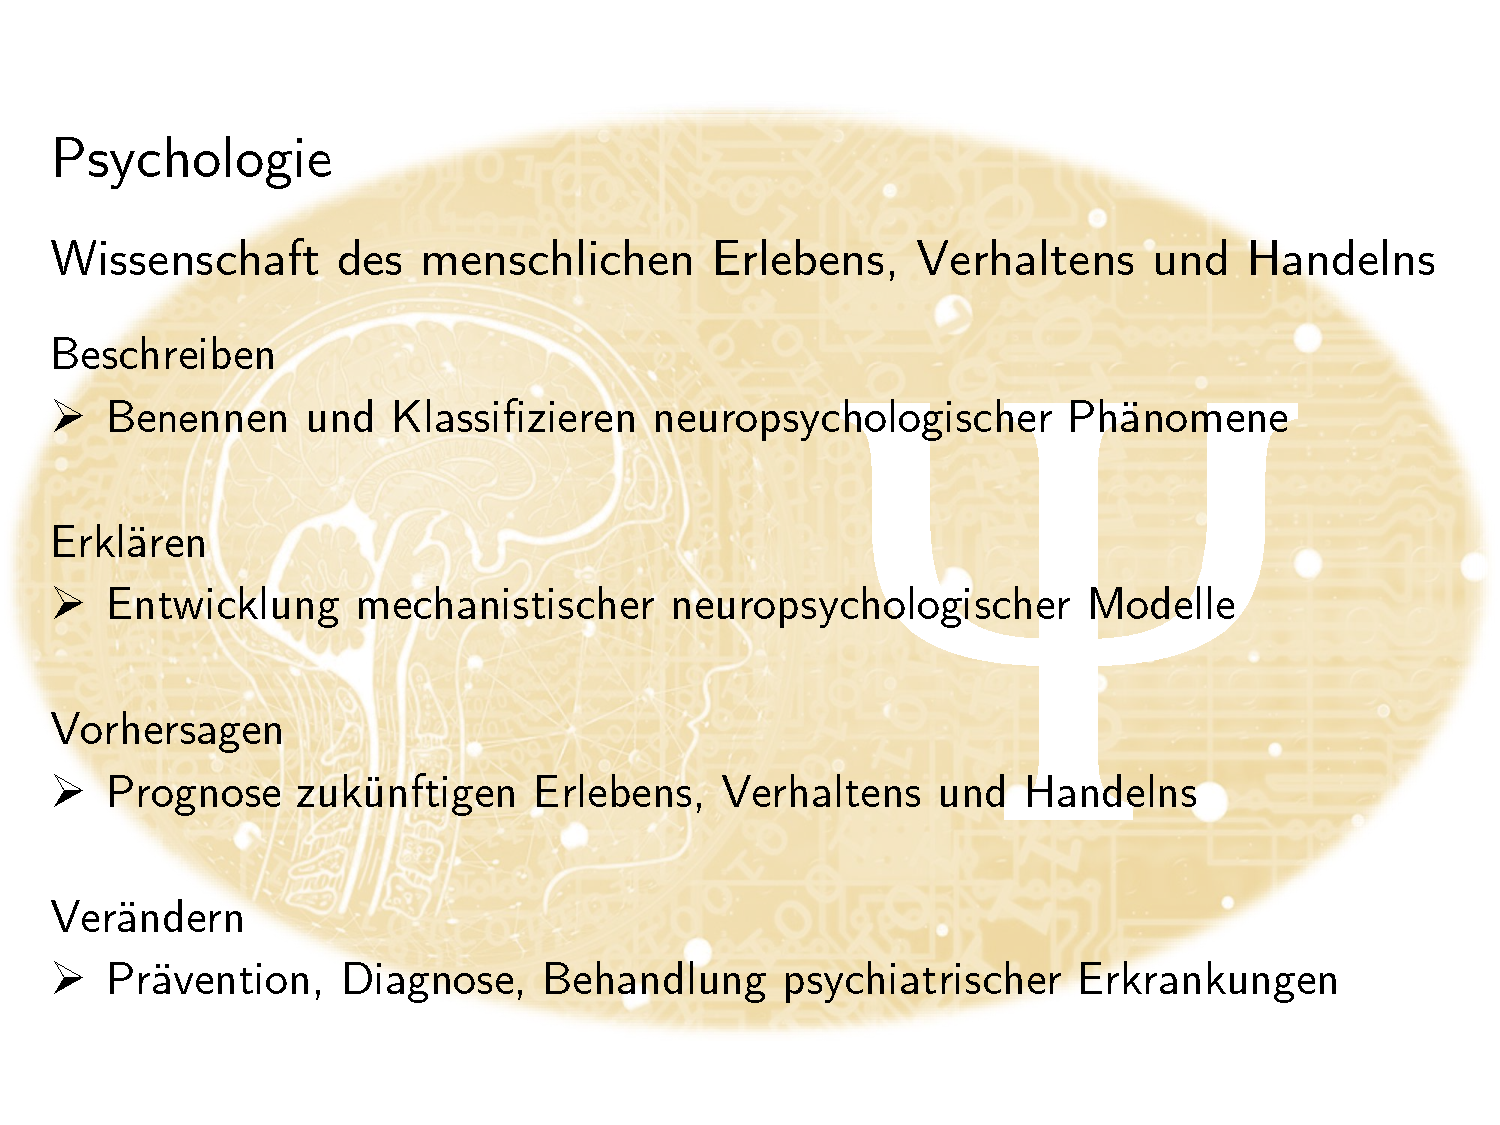
\includegraphics[width=1\linewidth]{2_Abbildungen/pfm_2_psychologie} \end{center}
\end{frame}

\begin{frame}{Einführung}
\protect\hypertarget{einfuxfchrung-1}{}
\begin{center}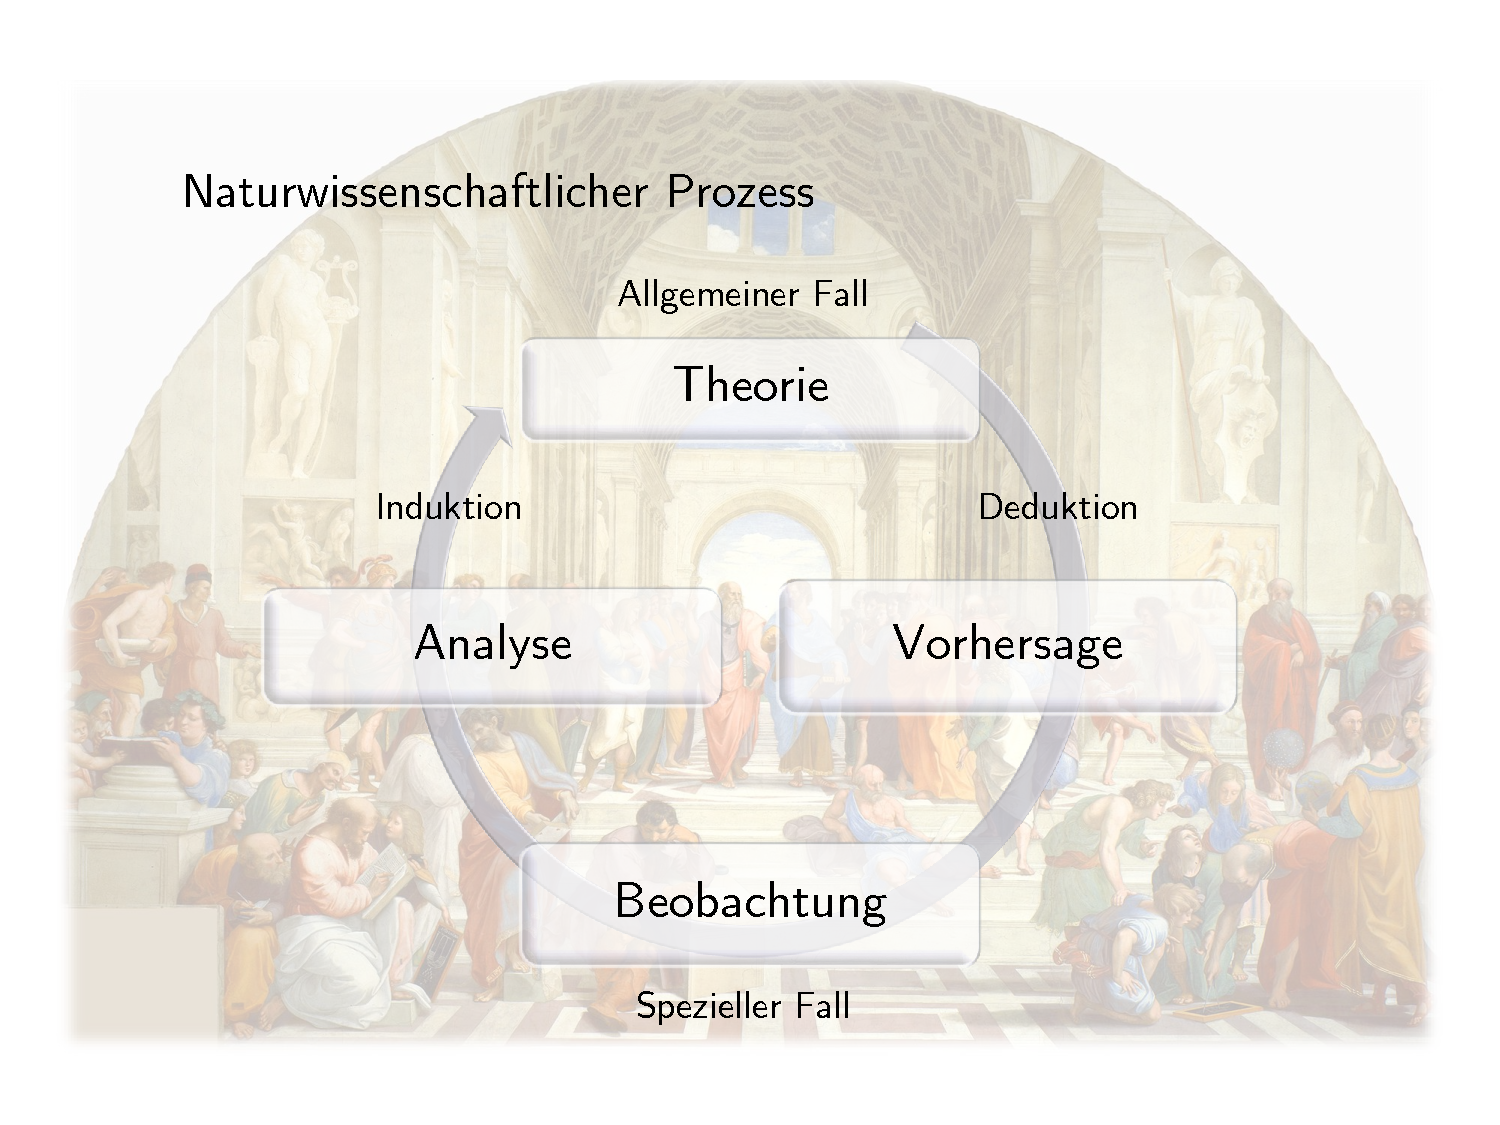
\includegraphics[width=1\linewidth]{2_Abbildungen/pfm_2_wissenschaft_prozess} \end{center}
\end{frame}

\begin{frame}{Einführung}
\protect\hypertarget{einfuxfchrung-2}{}
\large

Psychologische Datenwissenschaft

\begin{center}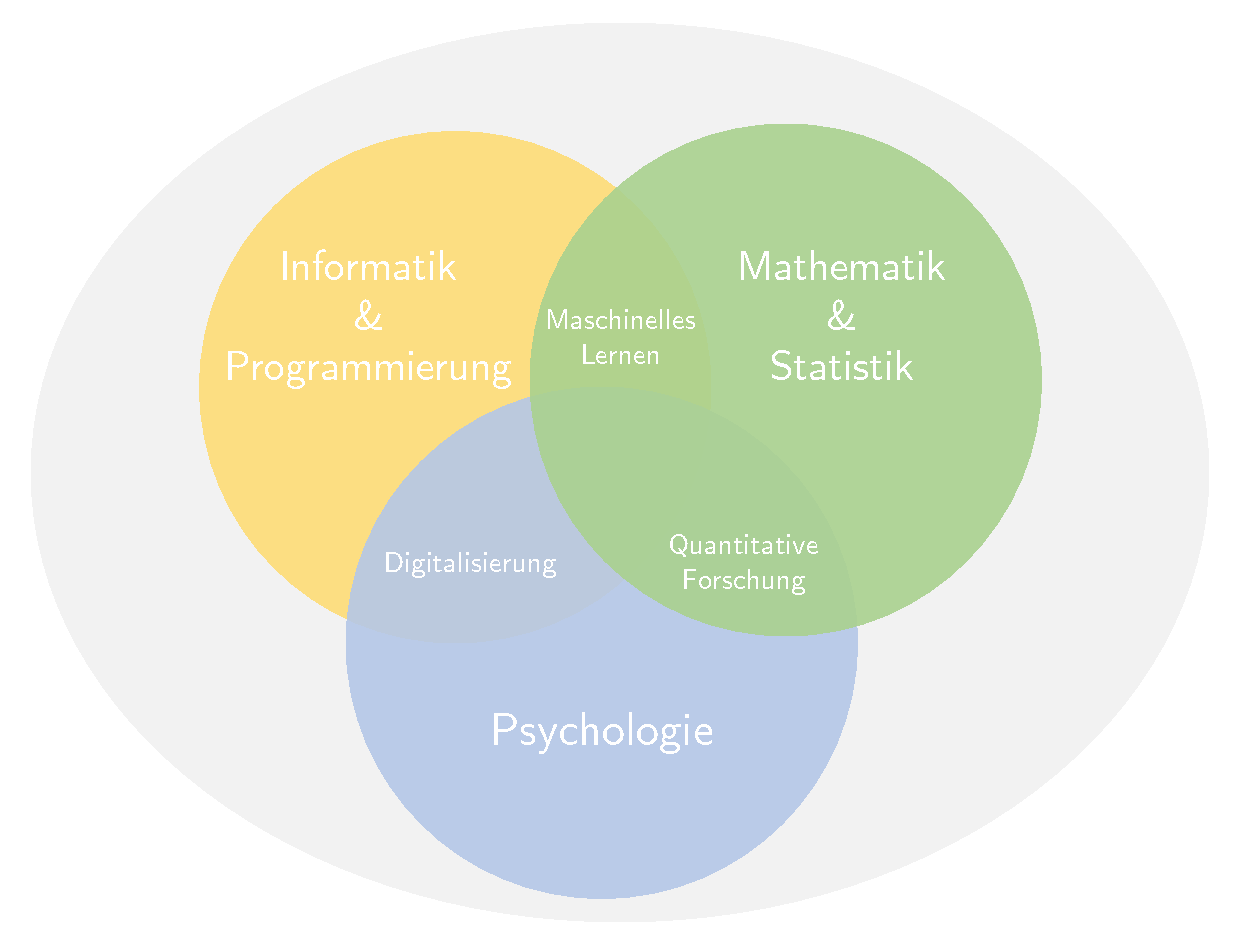
\includegraphics[width=0.8\linewidth]{2_Abbildungen/pfm_2_psychologische_datenwissenschaft} \end{center}
\end{frame}

\begin{frame}{Einführung}
\protect\hypertarget{einfuxfchrung-3}{}
\textcolor{darkblue}{Grundlagenforschung} \setstretch{1.8} \small

\begin{itemize}
\tightlist
\item
  Verstehen der mechanistischen Zusammenhänge eines Gegenstandbereichs.
\item
  Verstehen, wie und warum etwas funktioniert, wie es funktioniert.
\item
  Wissensbasierte intuitive Generation neuer mechanistischer Ideen.
\item
  Quantitative Überprüfung der generierten Ideen im empirischen Kontext.
\item
  Kommunikation und rationale Diskussion der Ideen und ihres empirischen
  Supports.
\end{itemize}

\normalsize

\textcolor{darkblue}{Anwendungsforschung} \small

\begin{itemize}
\tightlist
\item
  Verstehen, welche Form von Intervention ein gewünschtes Ergebnis
  hervorbringt.
\item
  Verstehen, wie etwas verändert werden kann ohne notwendig, zu
  verstehen, wie es funktioniert.
\item
  Wissensbasierte intuitive Generation neuer Interventionsformen.
\item
  Quantitative Überprüfung von Interventionen im empirischen Kontext.
\item
  Kommunikation und rationale Diskussion der Interventionen und ihres
  empirischen Supports.
\end{itemize}
\end{frame}

\begin{frame}{}
\protect\hypertarget{section-4}{}
\setstretch{3}
\large

Einführung

\textbf{Beispiele grundlagenorientierter psychologischer Forschung}

Beispiele anwendungsorientierter psychologischer Forschung

Selbstkontrollfragen
\end{frame}

\begin{frame}{Erklären und Vorhersagen menschlichen Verhaltens}
\protect\hypertarget{erkluxe4ren-und-vorhersagen-menschlichen-verhaltens}{}
\textcolor{darkblue}{Erklären und Vorhersagen menschlichen Verhaltens}
\vspace{2mm}

\begin{center}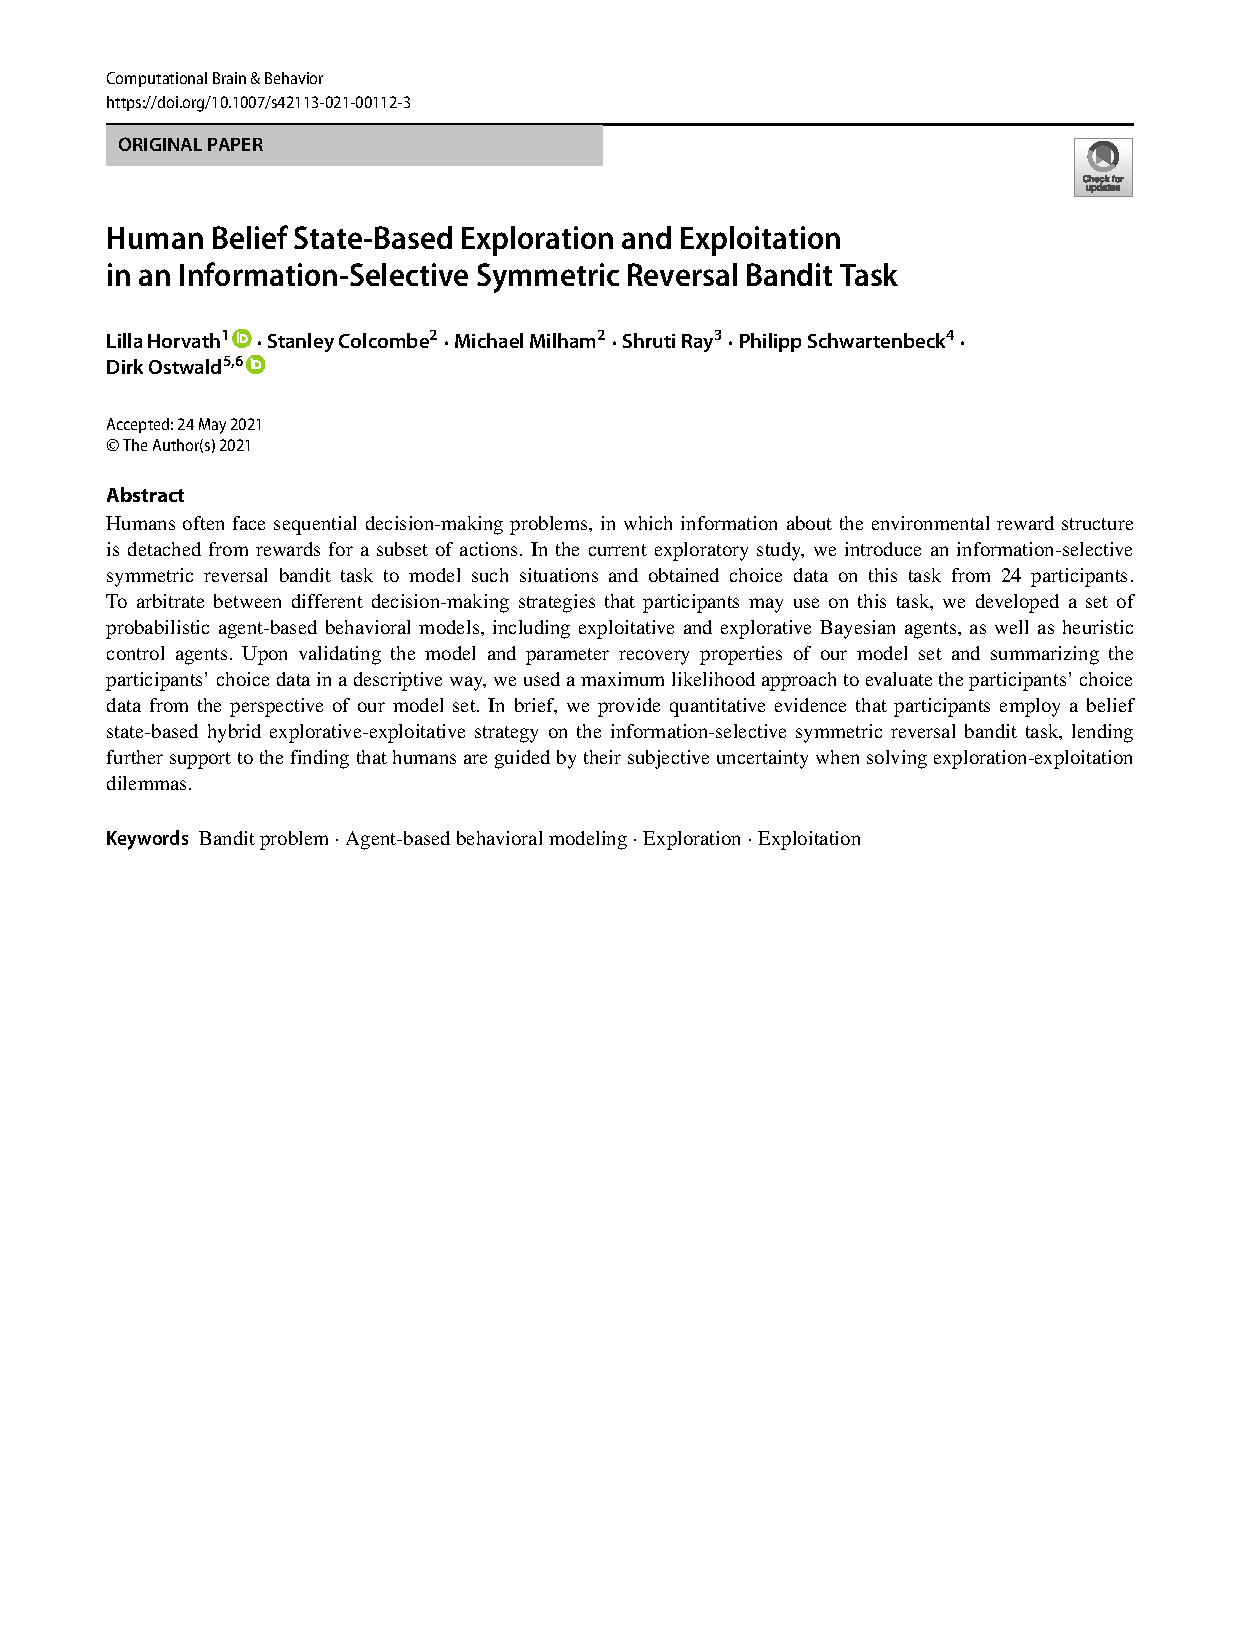
\includegraphics[width=0.8\linewidth]{2_Abbildungen/pfm_2_horvath_abstract} \end{center}

\flushright
\footnotesize

Horvath et al. (2021)
\end{frame}

\begin{frame}{Erklären und Vorhersagen menschlichen Verhalten}
\protect\hypertarget{erkluxe4ren-und-vorhersagen-menschlichen-verhalten}{}
\textcolor{darkblue}{Gegenstandsbereich und Phänomen}

\setstretch{1.8}

Menschen müssen oft Entscheidungen unter Unsicherheit treffen

Menschen müssen manchmal informations- und gewinnbringende Handlungen
abwägen

\begin{center}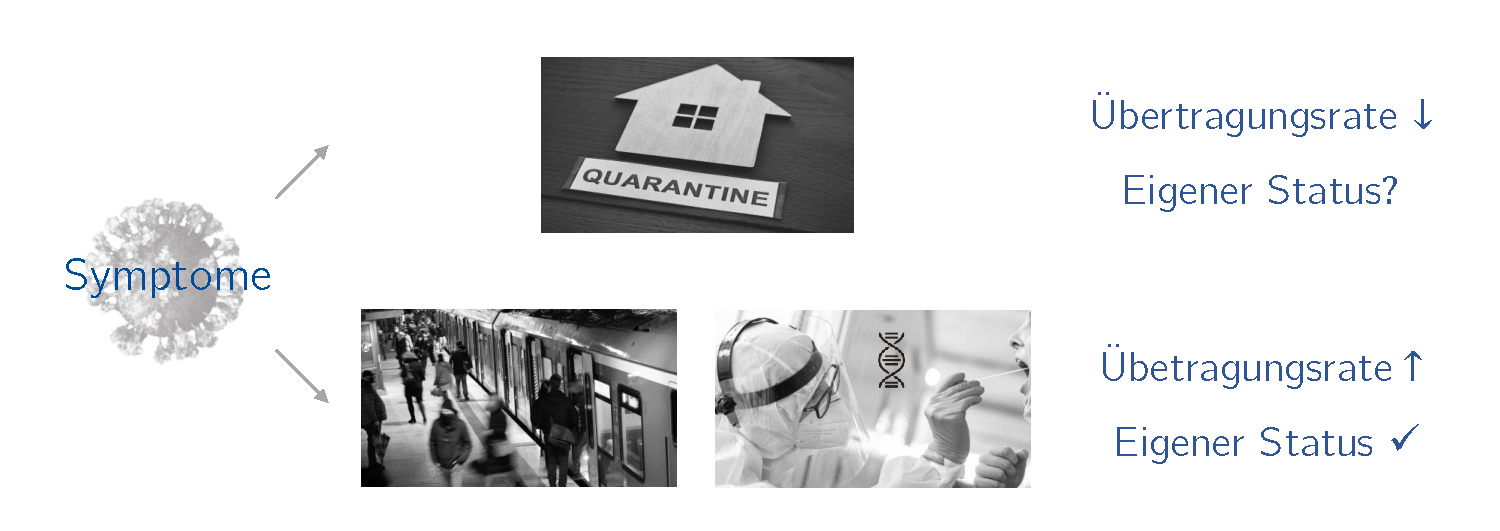
\includegraphics[width=0.8\linewidth]{2_Abbildungen/pfm_2_horvath_gegenstandsbereich} \end{center}

\begin{itemize}
\item
  Wie gehen Menschen dabei vor?
\item
  Wie lernen Menschen in solchen Situationen Entscheidungen zu treffen?
\end{itemize}

\flushright
\footnotesize

Horvath et al. (2021)
\end{frame}

\begin{frame}{Beispiel}
\protect\hypertarget{beispiel}{}
\textcolor{darkblue}{Experimentelle Simulation} \vfill
Verhaltensdatenaufnahme

\begin{center}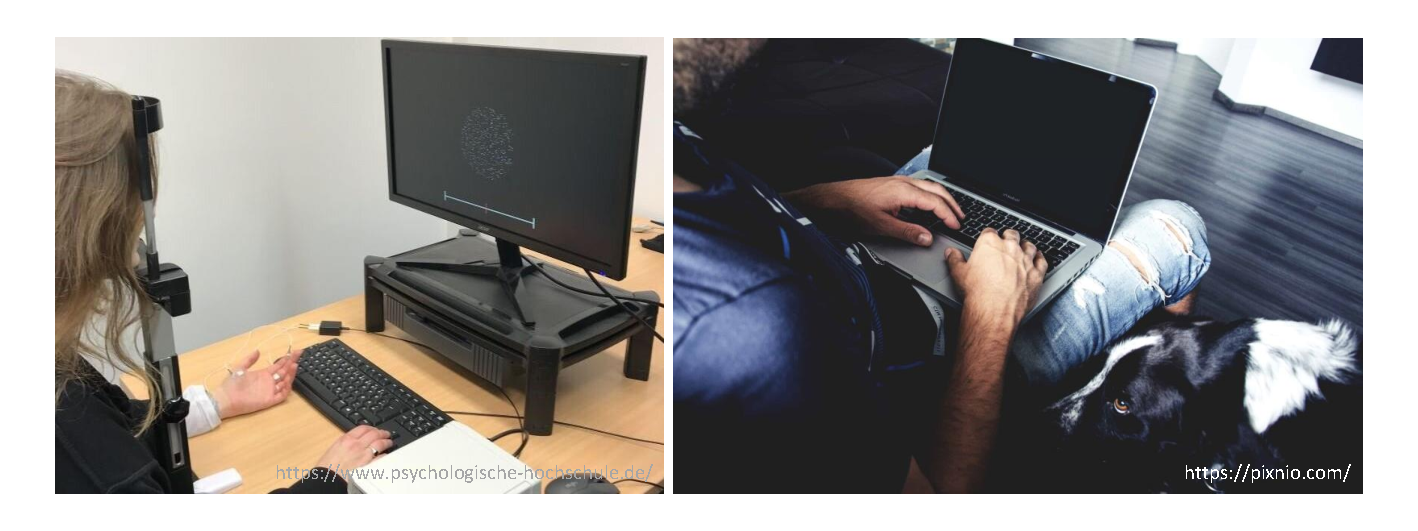
\includegraphics[width=1\linewidth]{2_Abbildungen/pfm_2_verhaltensdatenaufnahme} \end{center}
\vfill

\flushright
\footnotesize

Horvath et al. (2021)
\end{frame}

\begin{frame}{Beispiel}
\protect\hypertarget{beispiel-1}{}
\textcolor{darkblue}{Experimentelle Simulation} \vspace{-2mm}

\begin{center}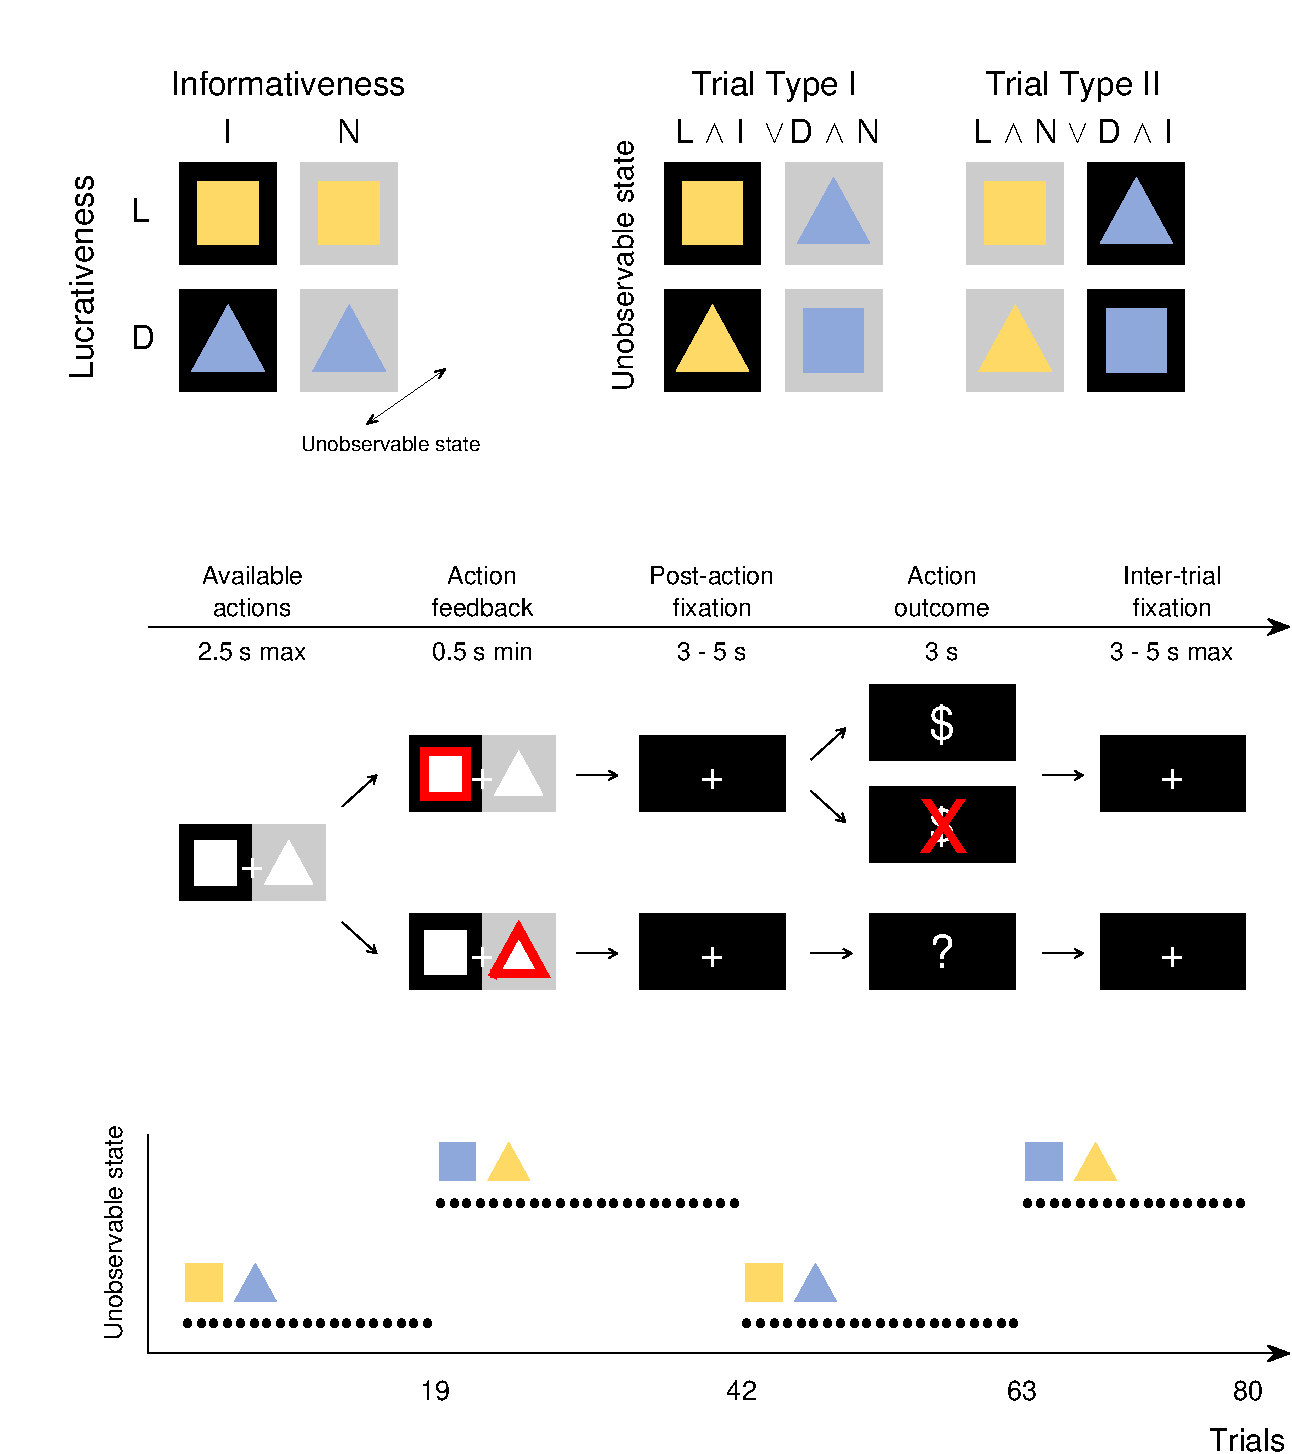
\includegraphics[width=0.55\linewidth]{2_Abbildungen/pfm_2_horvath_experimentelle_simulation} \end{center}

\flushright
\footnotesize

Horvath et al. (2021)
\end{frame}

\begin{frame}{Erklären und Vorhersagen menschlichen Verhalten}
\protect\hypertarget{erkluxe4ren-und-vorhersagen-menschlichen-verhalten-1}{}
\textcolor{darkblue}{Theorie}

Künstliche Intelligenz - Artificial Agent

\begin{equation*}
\mbox{M}_{\mbox{\tiny Agent}}
:= (S,A,R,O,p(s_1^1),p(s_{t+1}^1|s_t^{1}), p^{a_t}(o_t|s_t^1), p^{a_t}(r_t|s_t^1), v, d)
\end{equation*} \vspace{-5mm}

\begin{itemize}
\itemsep2mm
\item Dynamisches handlungsabhängiges generatives Modell
\vspace{-3mm}
\begin{equation*}
p^{a_{1:T}}(s_{1:T}^1,o_{1:T})
= p(s_1^1) \prod_{t=1}^T p^{a_t}(o_t|s_t^1)p(s_{t+1}^1|s_t^{1})
\end{equation*}
\vspace{-5mm}
\item Handlungsabhängige Zustandsschätzung (Belief State)
\begin{footnotesize}
\begin{equation*}
p^{a_{1:t-1}}(s_t^1|o_{1:t-1})
= \frac{\sum_{s_{t-1}^1} p(s_t^1|s_{t-1}^1)p^{a_{t-1}}(o_{t-1}|s_{t-1}^1)p^{a_{1:t-2}}(s_{t-1}^1|o_{1:t-2})}
       {\sum_{s_t^1}\sum_{s_{t-1}^1} p(s_t^1|s_{t-1}^1)p^{a_{t-1}}(o_{t-1}|s_{t-1}^1)p^{a_{1:t-2}}(s_{t-1}^1|o_{1:t-2})}
\end{equation*}
\end{footnotesize}
\end{itemize}

\flushright
\footnotesize

Horvath et al. (2021)
\end{frame}

\begin{frame}{Erklären und Vorhersagen menschlichen Verhalten}
\protect\hypertarget{erkluxe4ren-und-vorhersagen-menschlichen-verhalten-2}{}
\textcolor{darkblue}{Theorie}

Künstliche Intelligenz - Artificial Agent

\begin{equation*}
\mbox{M}_{\mbox{\tiny Agent}}
:= (S,A,R,O,p(s_1^1),p(s_{t+1}^1|s_t^{1}), p^{a_t}(o_t|s_t^1), p^{a_t}(r_t|s_t^1), v, d)
\end{equation*} \vspace{-5mm}

\begin{itemize}
\itemsep2mm
\item Handlungswertungsfunktion
\begin{equation*}
v : A \times [0,1] \to \mathbb{R}, (a,b) \mapsto v(a,b)
\end{equation*}
\item Entscheidungsfunktion
\begin{equation*}
d : \mathbb{R} \to A,  v(\cdot,b) \mapsto d(v(\cdot,b)) := \argmax_{a \in A} v(a,b)
\end{equation*}
\end{itemize}

\flushright
\footnotesize

Horvath et al. (2021)
\end{frame}

\begin{frame}{Erklären und Vorhersagen menschlichen Verhalten}
\protect\hypertarget{erkluxe4ren-und-vorhersagen-menschlichen-verhalten-3}{}
\textcolor{darkblue}{Theorievarianten}

\small

\textcolor{darkblue}{\textbf{A1}  $\vert$} Gewinnmaximierender Agent
\begin{equation*}
v_{\mbox{\tiny A1}}(a,b)
:=     b\mathbb{E}_{p^{a}(r_t|s_t^1 = 1)}(r_t)
 + (1-b)\mathbb{E}_{p^{a}(r_t|s_t^1 = 2)}(r_t)
\end{equation*} \(\Rightarrow\) Erwartete Belohung von \(a\) unter
momentaner Zustandsschätzug \(b_t = b\)

\textcolor{darkblue}{\textbf{A2} $\vert$} Informationsmaximierender
Agent

\begin{small}
\begin{equation*}
v_{\mbox{\tiny A2}}(a,b)
:=
\sum_{o_t} p_{a_{1:t-1},a_t = a} (o_t|o_{1:t-1})
\mbox{KL}\left(p_{a_{t-1},a_t = a}(s_{t+1}^1|o_{1:t-1},o_t) \Vert p_{a_{1:t-1}}(s_t^1|o_{1:t-1}) \right)
\end{equation*}
\end{small}

\(\Rightarrow\) Erwartete Bayesianische Überaschung von \(a\) unter
momentaner Zustandsschätzug \(b_t = b\)

\textcolor{darkblue}{\textbf{A3} $\vert$} Gewinn- und
informationsmaximierender Agent \begin{equation*}
v_{\mbox{\tiny A3}}(a,b)
:= \lambda v_{\mbox{\tiny A1}}(a,b) +  (1-\lambda) v_{\mbox{\tiny A2}}(a,b)
\end{equation*}

\(\Rightarrow\) Gewichtete Kombination der beiden Theoriealternativen

\flushright
\footnotesize

Horvath et al. (2021)
\end{frame}

\begin{frame}{Erklären und Vorhersagen menschlichen Verhalten}
\protect\hypertarget{erkluxe4ren-und-vorhersagen-menschlichen-verhalten-4}{}
\textcolor{darkblue}{Datenvorhersage} \vspace{2mm}

\begin{center}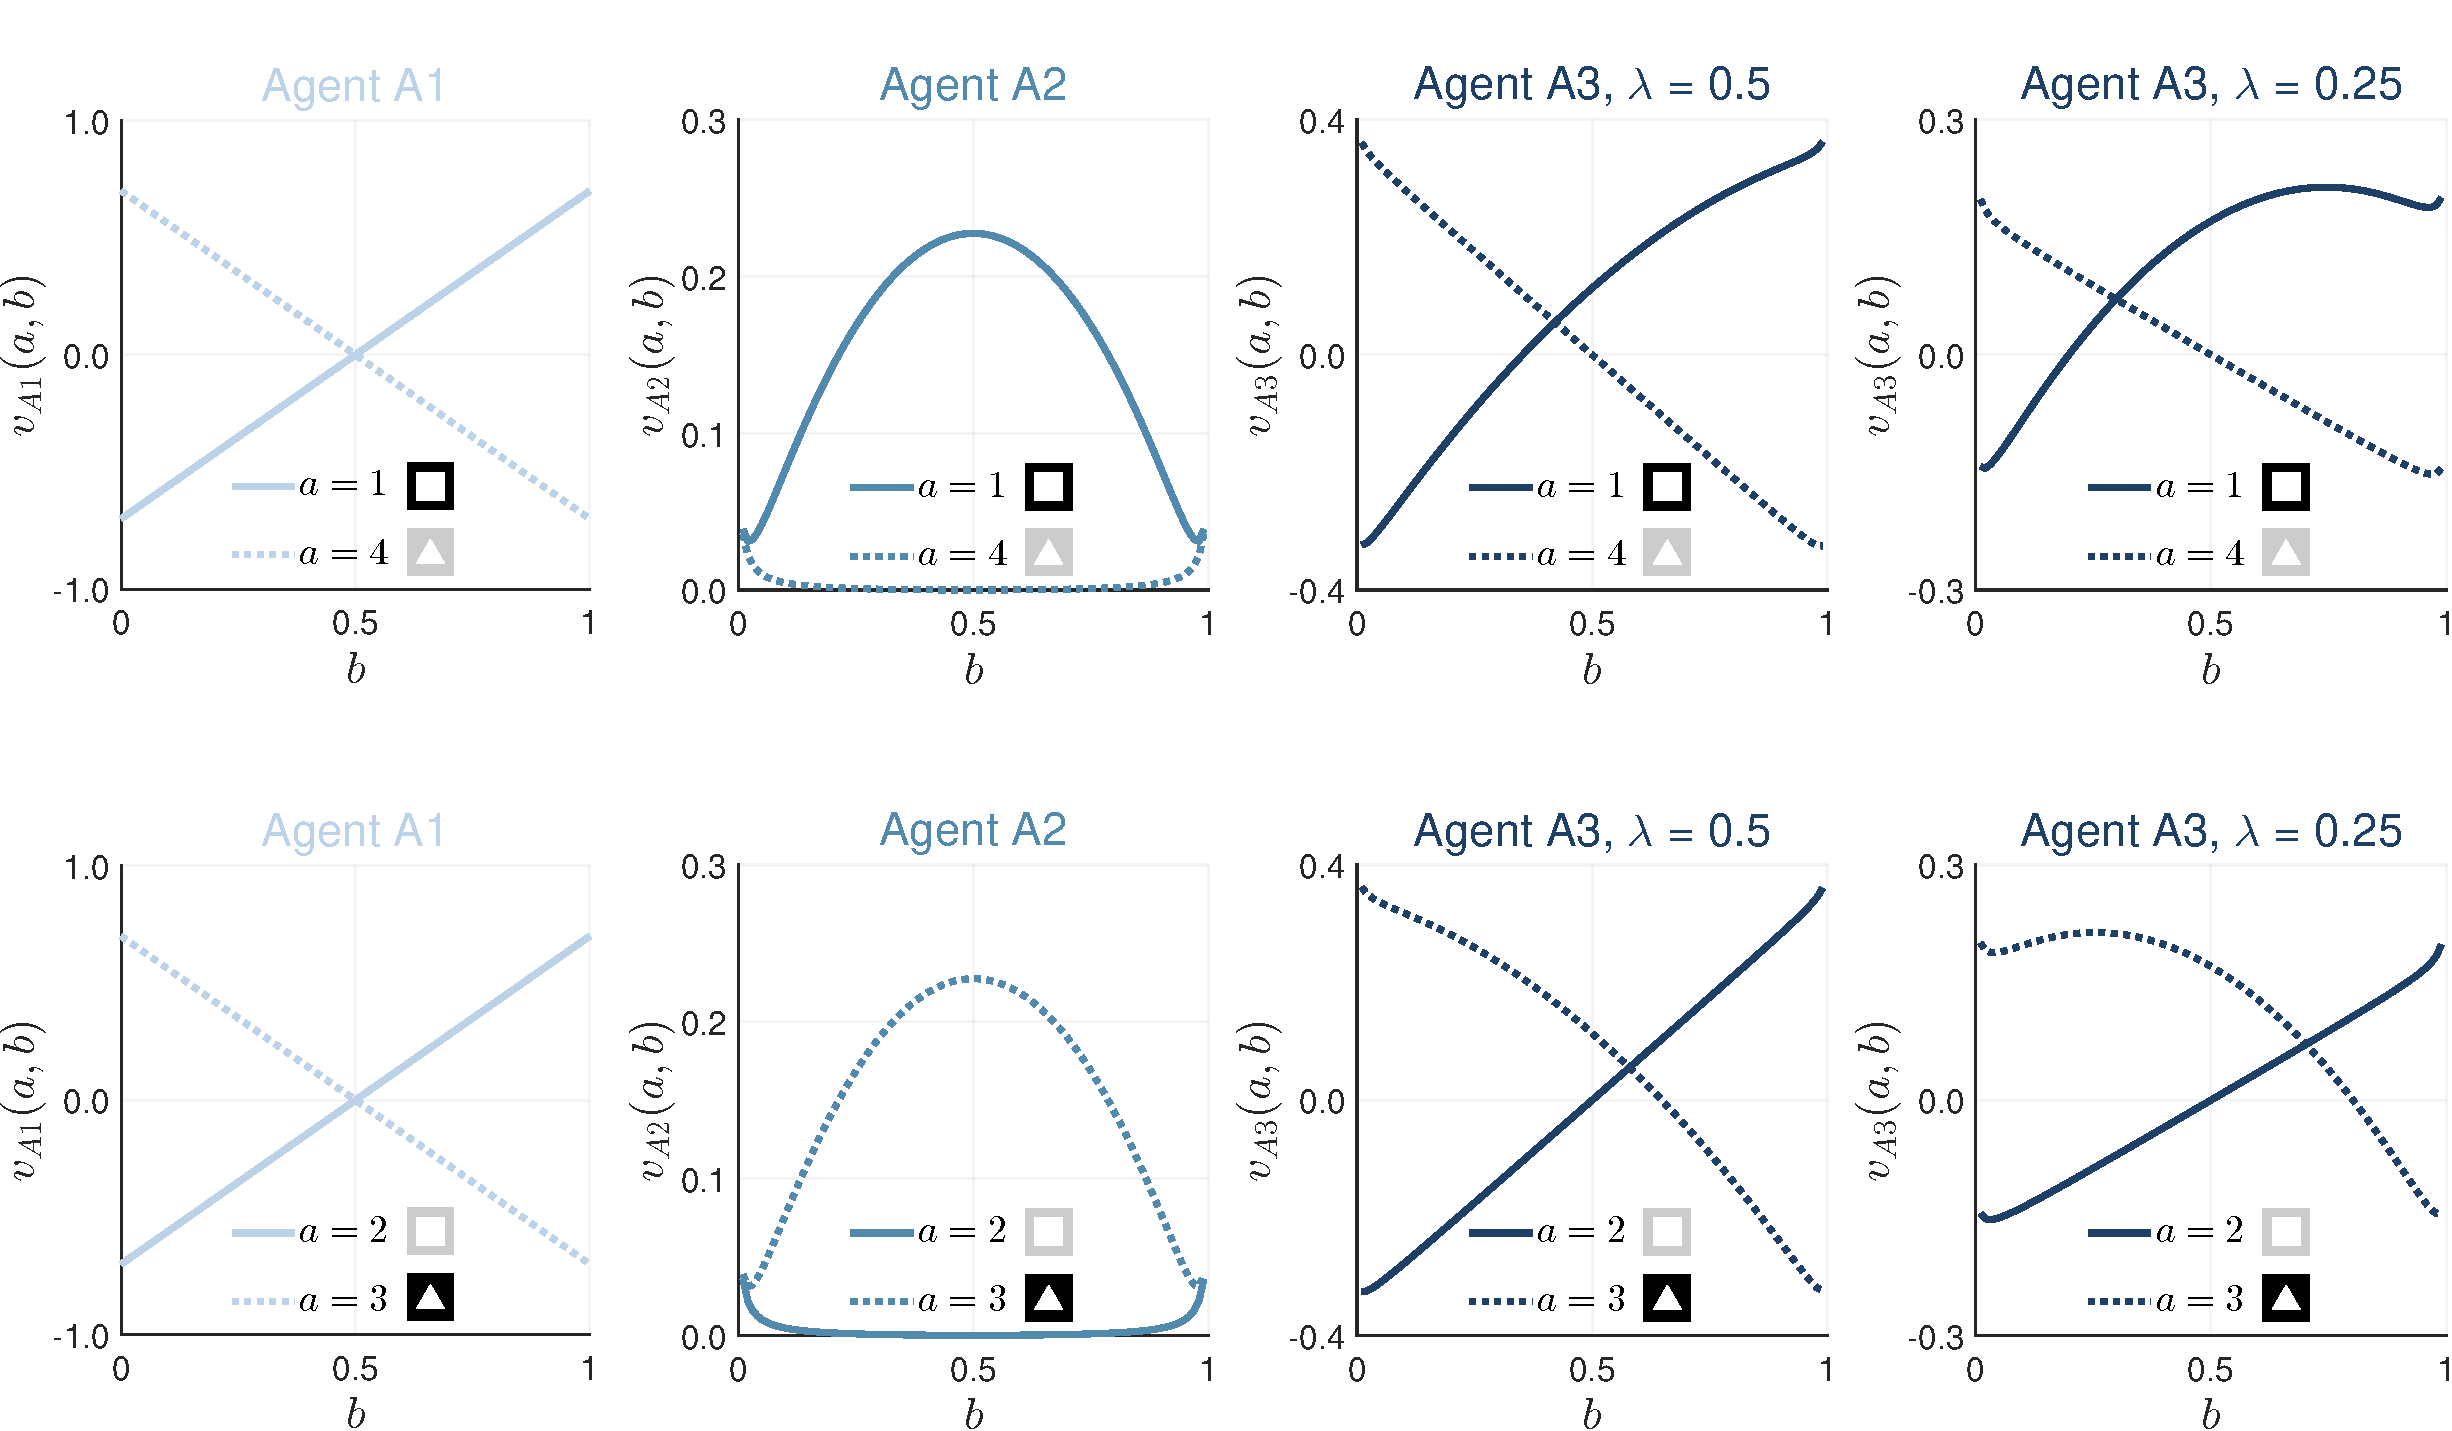
\includegraphics[width=0.8\linewidth]{2_Abbildungen/pfm_2_horvath_datenvorhersage} \end{center}

\flushright
\footnotesize

Horvath et al. (2021)
\end{frame}

\begin{frame}{Beispiel}
\protect\hypertarget{beispiel-2}{}
\textcolor{darkblue}{Datenanalyse}

\begin{center}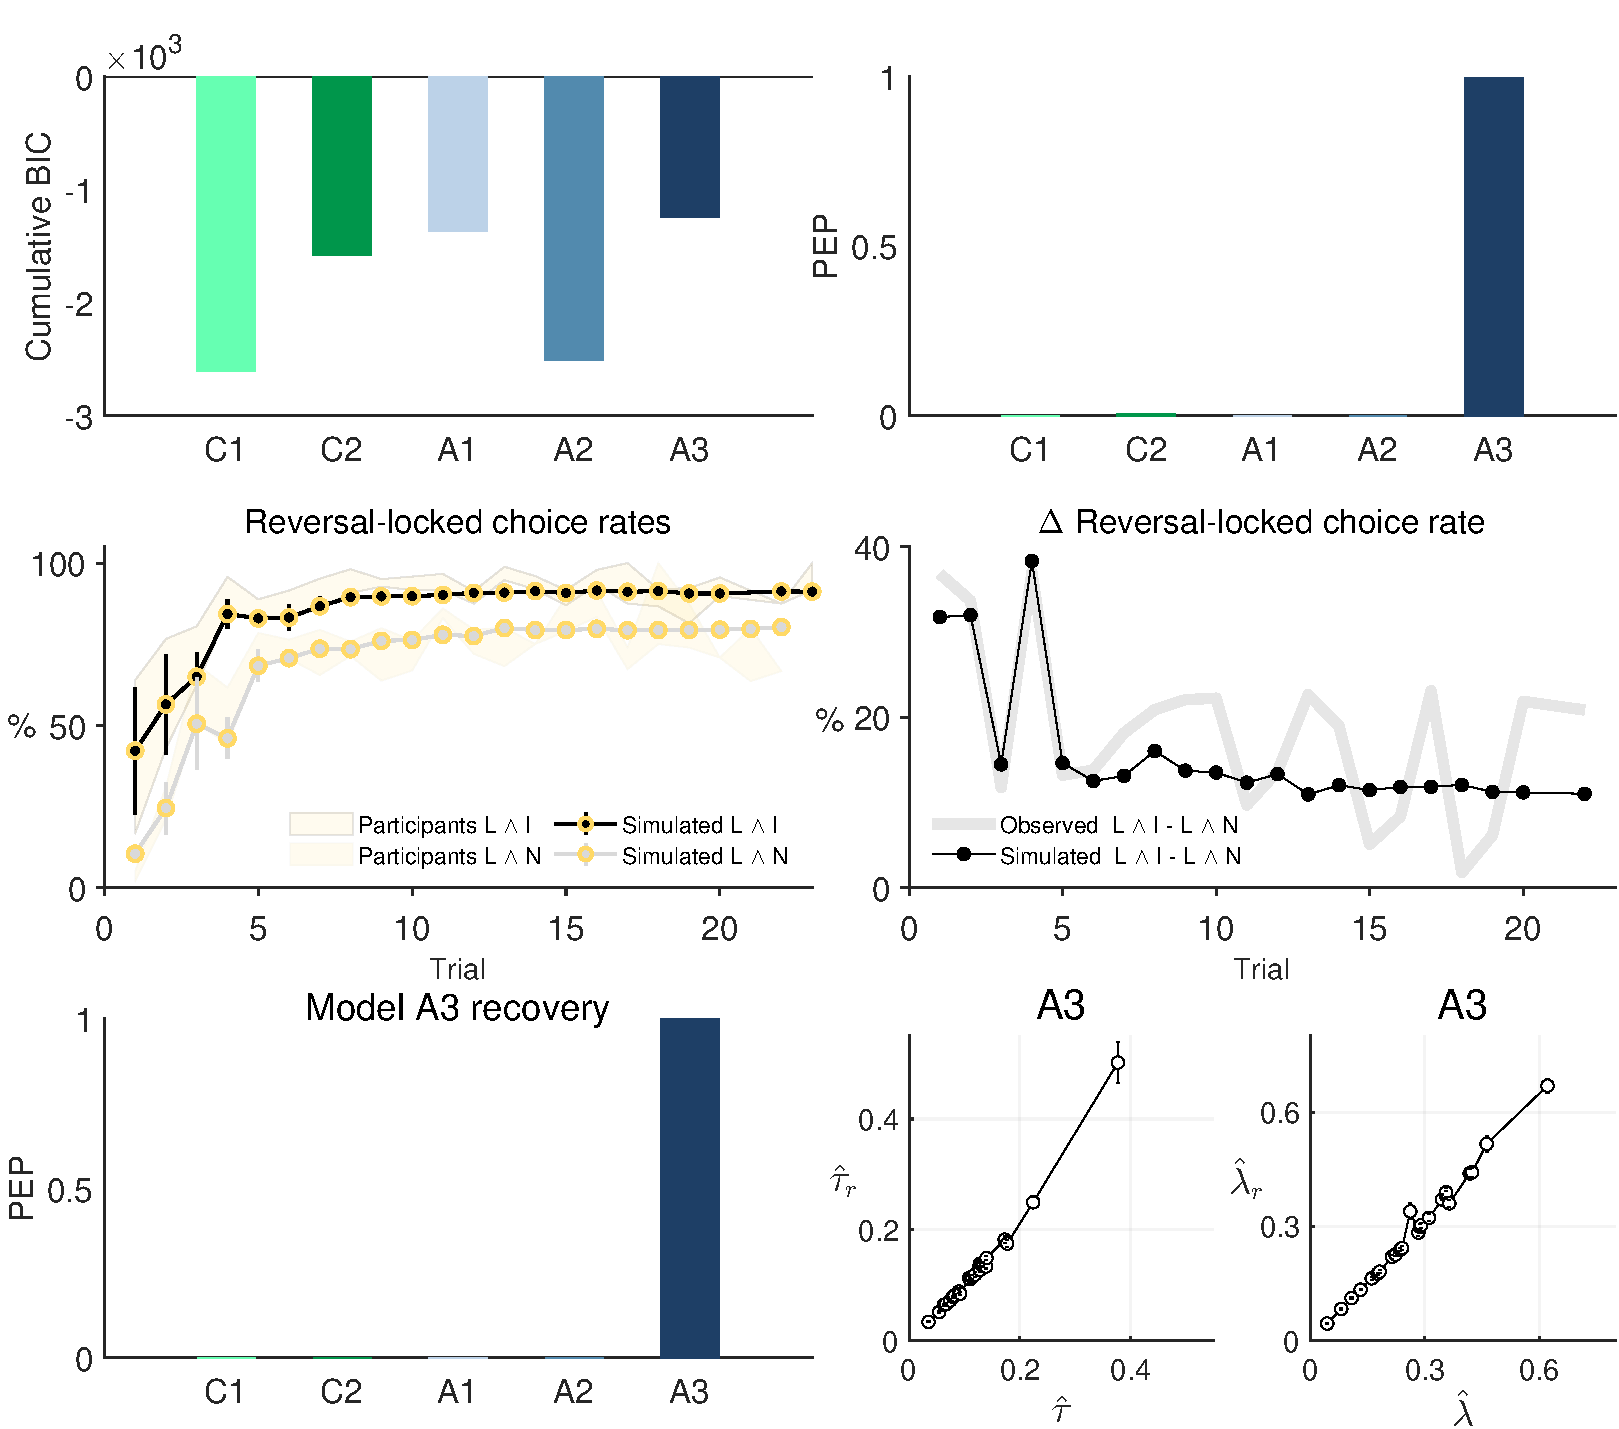
\includegraphics[width=0.65\linewidth]{2_Abbildungen/pfm_2_horvath_datenanalyse} \end{center}

\flushright
\footnotesize

Horvath et al. (2021)
\end{frame}

\begin{frame}{Entwicklung mechanistischer neuropsychologischer Modelle}
\protect\hypertarget{entwicklung-mechanistischer-neuropsychologischer-modelle}{}
\textcolor{darkblue}{Entwicklung mechanistischer neuropsychologischer Modelle}
\vspace{2mm}

\begin{center}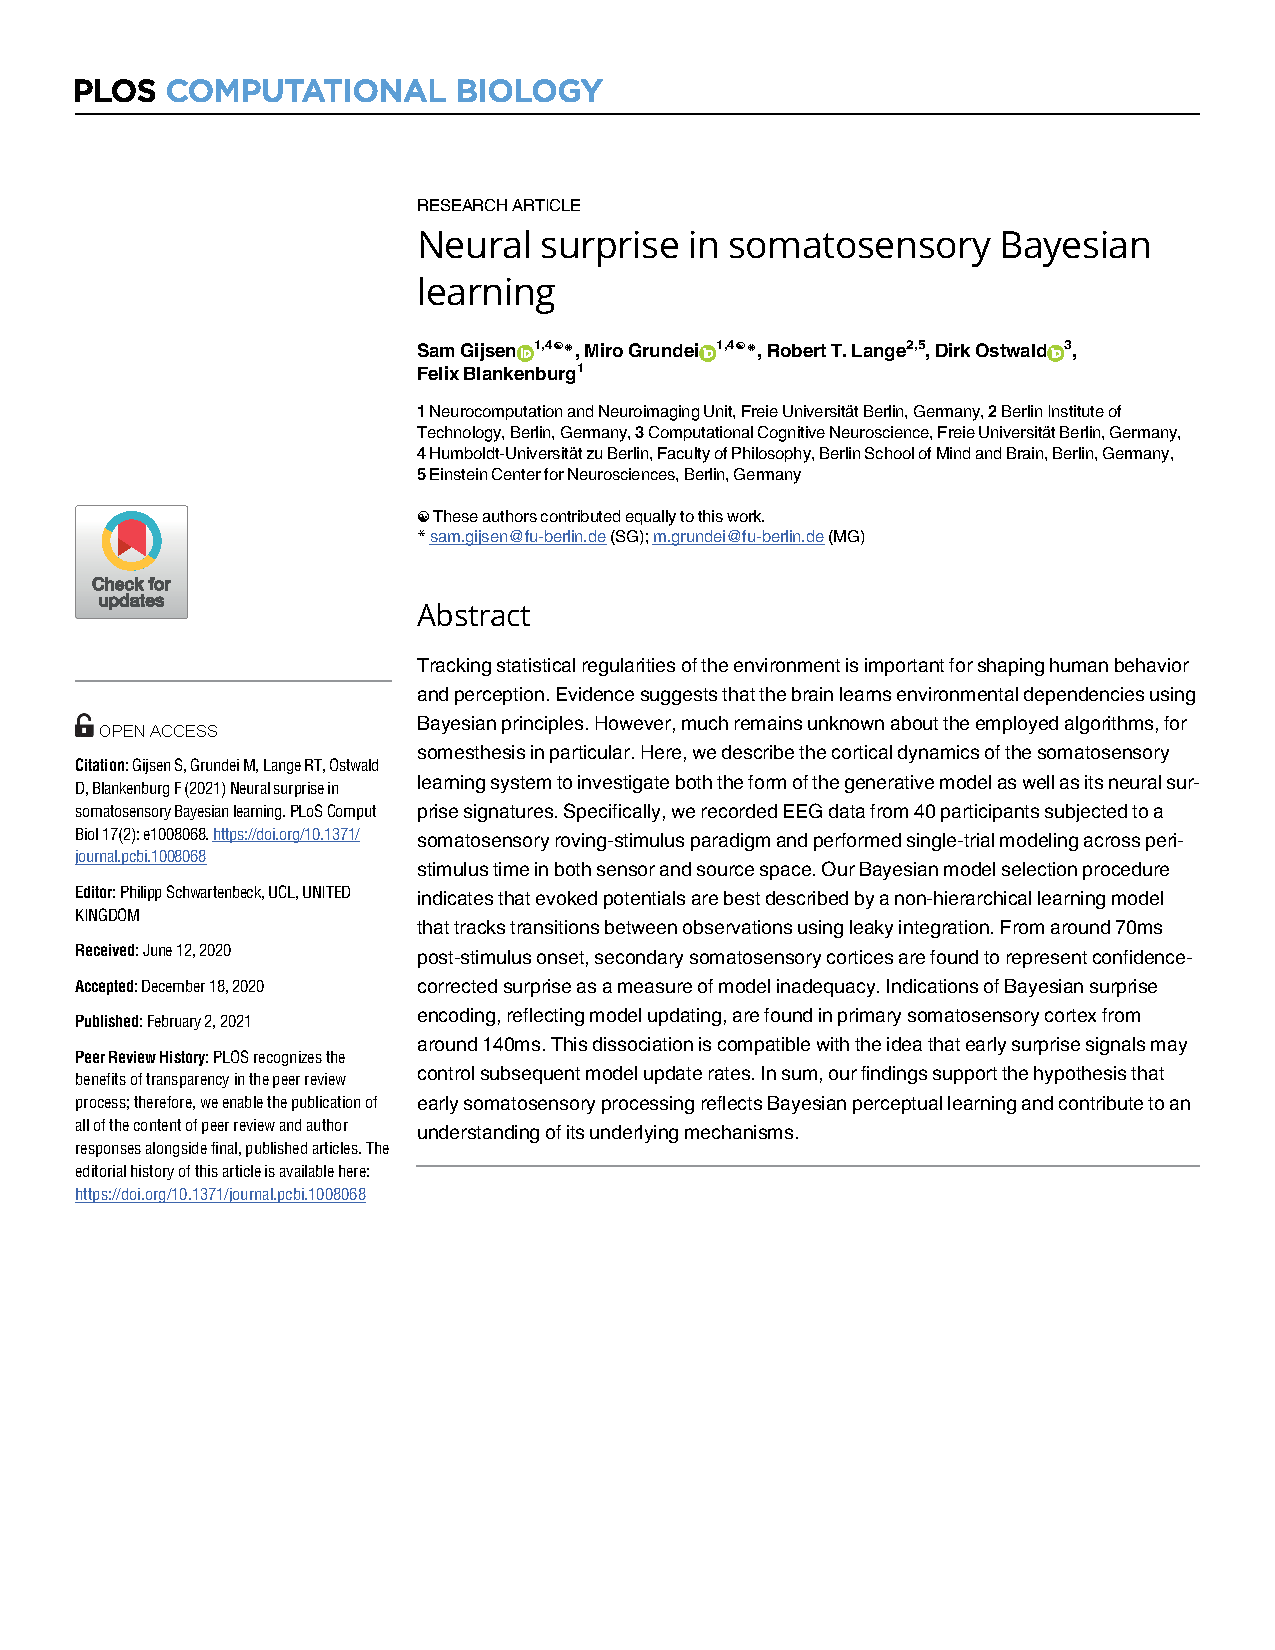
\includegraphics[width=0.6\linewidth]{2_Abbildungen/pfm_2_gijsen_abstract} \end{center}
\flushright
\footnotesize

Gijsen et al. (2021)
\end{frame}

\begin{frame}{Entwicklung mechanistischer neuropsychologischer Modelle}
\protect\hypertarget{entwicklung-mechanistischer-neuropsychologischer-modelle-1}{}
\vspace{2mm}

\textcolor{darkblue}{Theorie | The Bayesian Brain Hypothesis}
\vspace{-2mm}

\begin{center}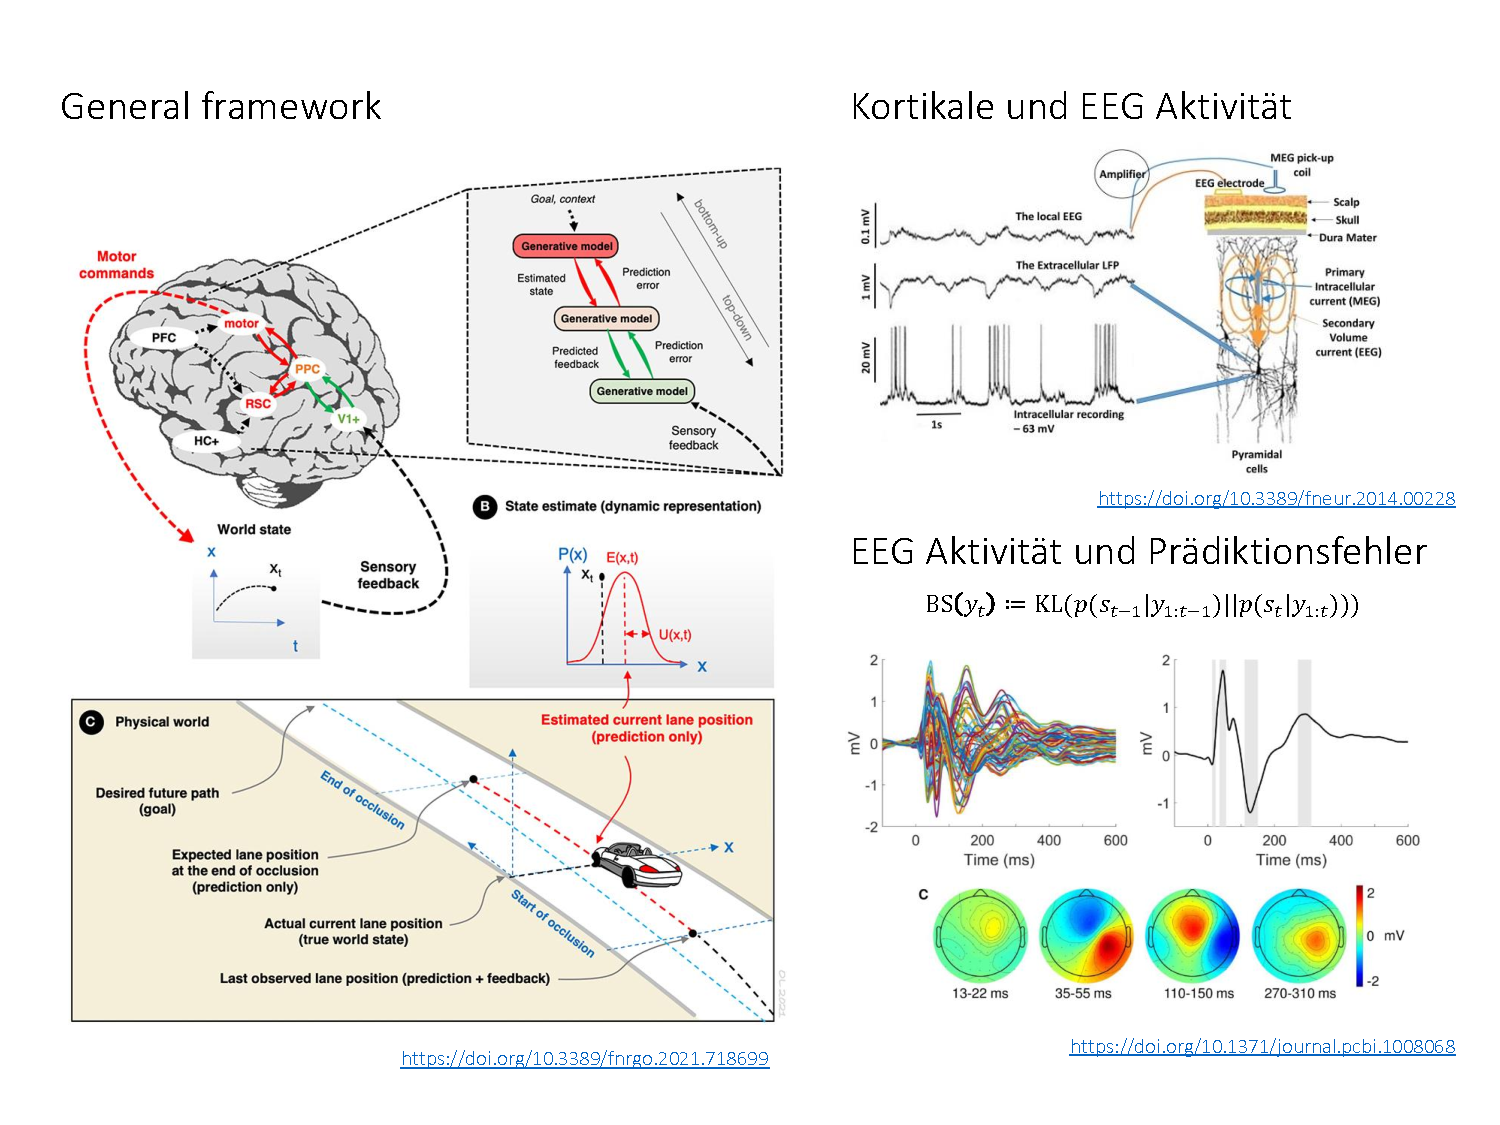
\includegraphics[width=0.9\linewidth]{2_Abbildungen/pfm_2_bayesian_brain_hypothesis} \end{center}
\vspace{-3mm}
\flushright
\footnotesize

Helmholtz (1867), Friston (2005), Ostwald et al. (2012), Gijsen et al.
(2021)
\end{frame}

\begin{frame}{Entwicklung mechanistischer neuropsychologischer Modelle}
\protect\hypertarget{entwicklung-mechanistischer-neuropsychologischer-modelle-2}{}
\textcolor{darkblue}{Experimentelle Simulation} \vfill

\begin{center}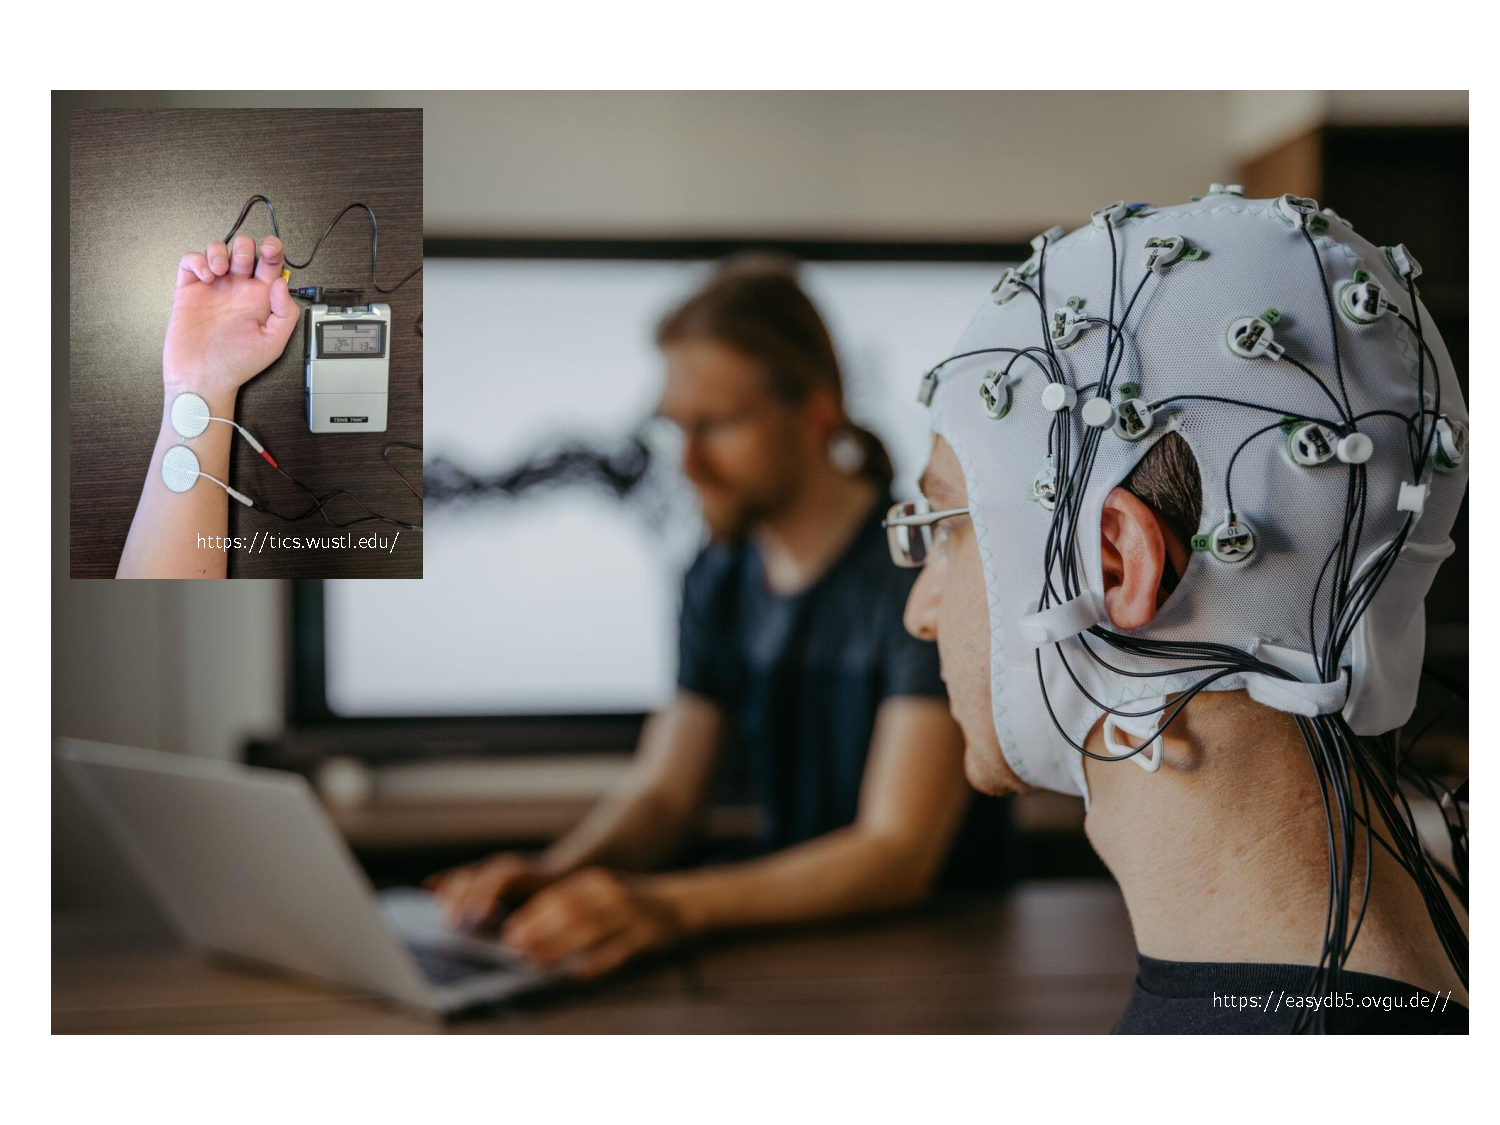
\includegraphics[width=0.7\linewidth]{2_Abbildungen/pfm_2_somatosensation_eeg} \end{center}
\vfill

\flushright
\footnotesize

Ostwald et al. (2012), Gijsen et al. (2021)
\end{frame}

\begin{frame}{Entwicklung mechanistischer neuropsychologischer Modelle}
\protect\hypertarget{entwicklung-mechanistischer-neuropsychologischer-modelle-3}{}
\textcolor{darkblue}{Experimentelle Simulation} \vfill

\begin{center}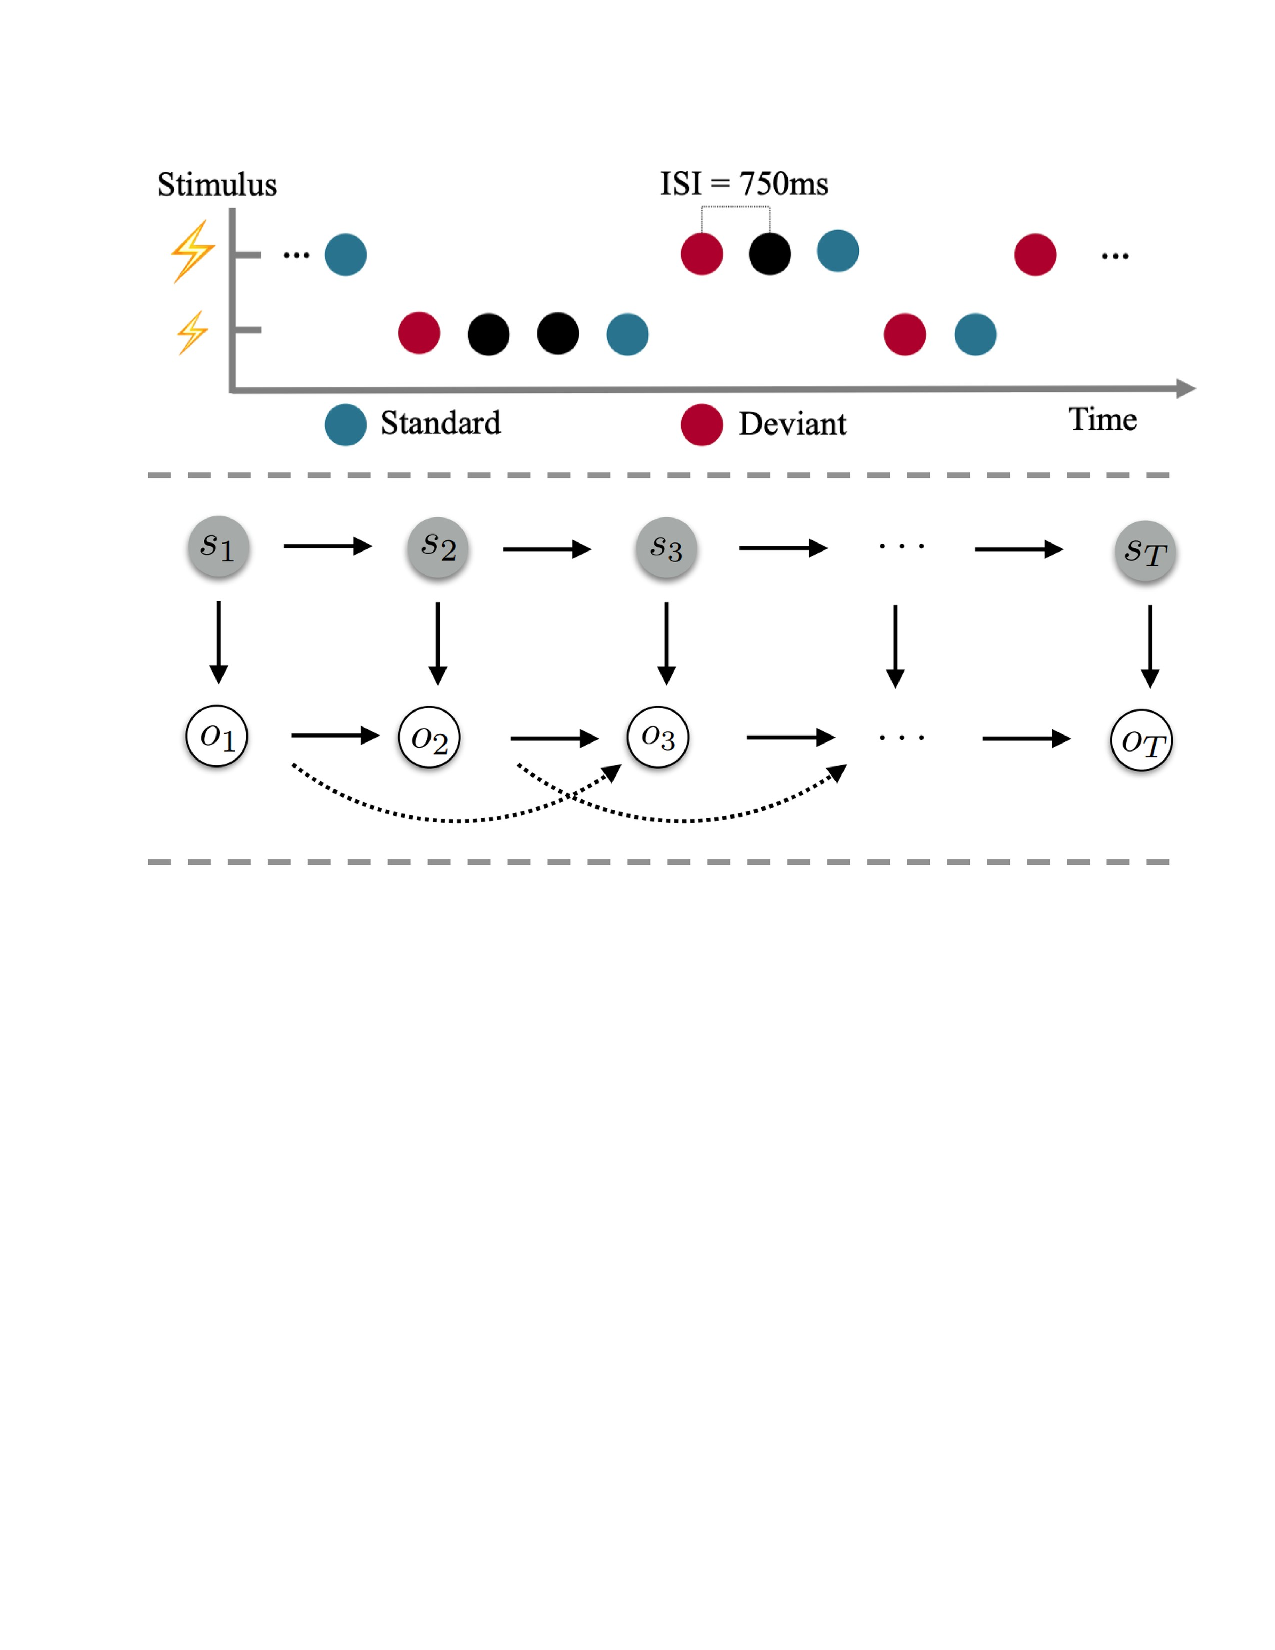
\includegraphics[width=0.7\linewidth]{2_Abbildungen/pfm_2_gijsen_experimentelle_simulation} \end{center}
\vfill
\flushright
\footnotesize

Ostwald et al. (2012), Gijsen et al. (2021)
\end{frame}

\begin{frame}{Entwicklung mechanistischer neuropsychologischer Modelle}
\protect\hypertarget{entwicklung-mechanistischer-neuropsychologischer-modelle-4}{}
\textcolor{darkblue}{Theorie} \vspace{-2mm}

\begin{center}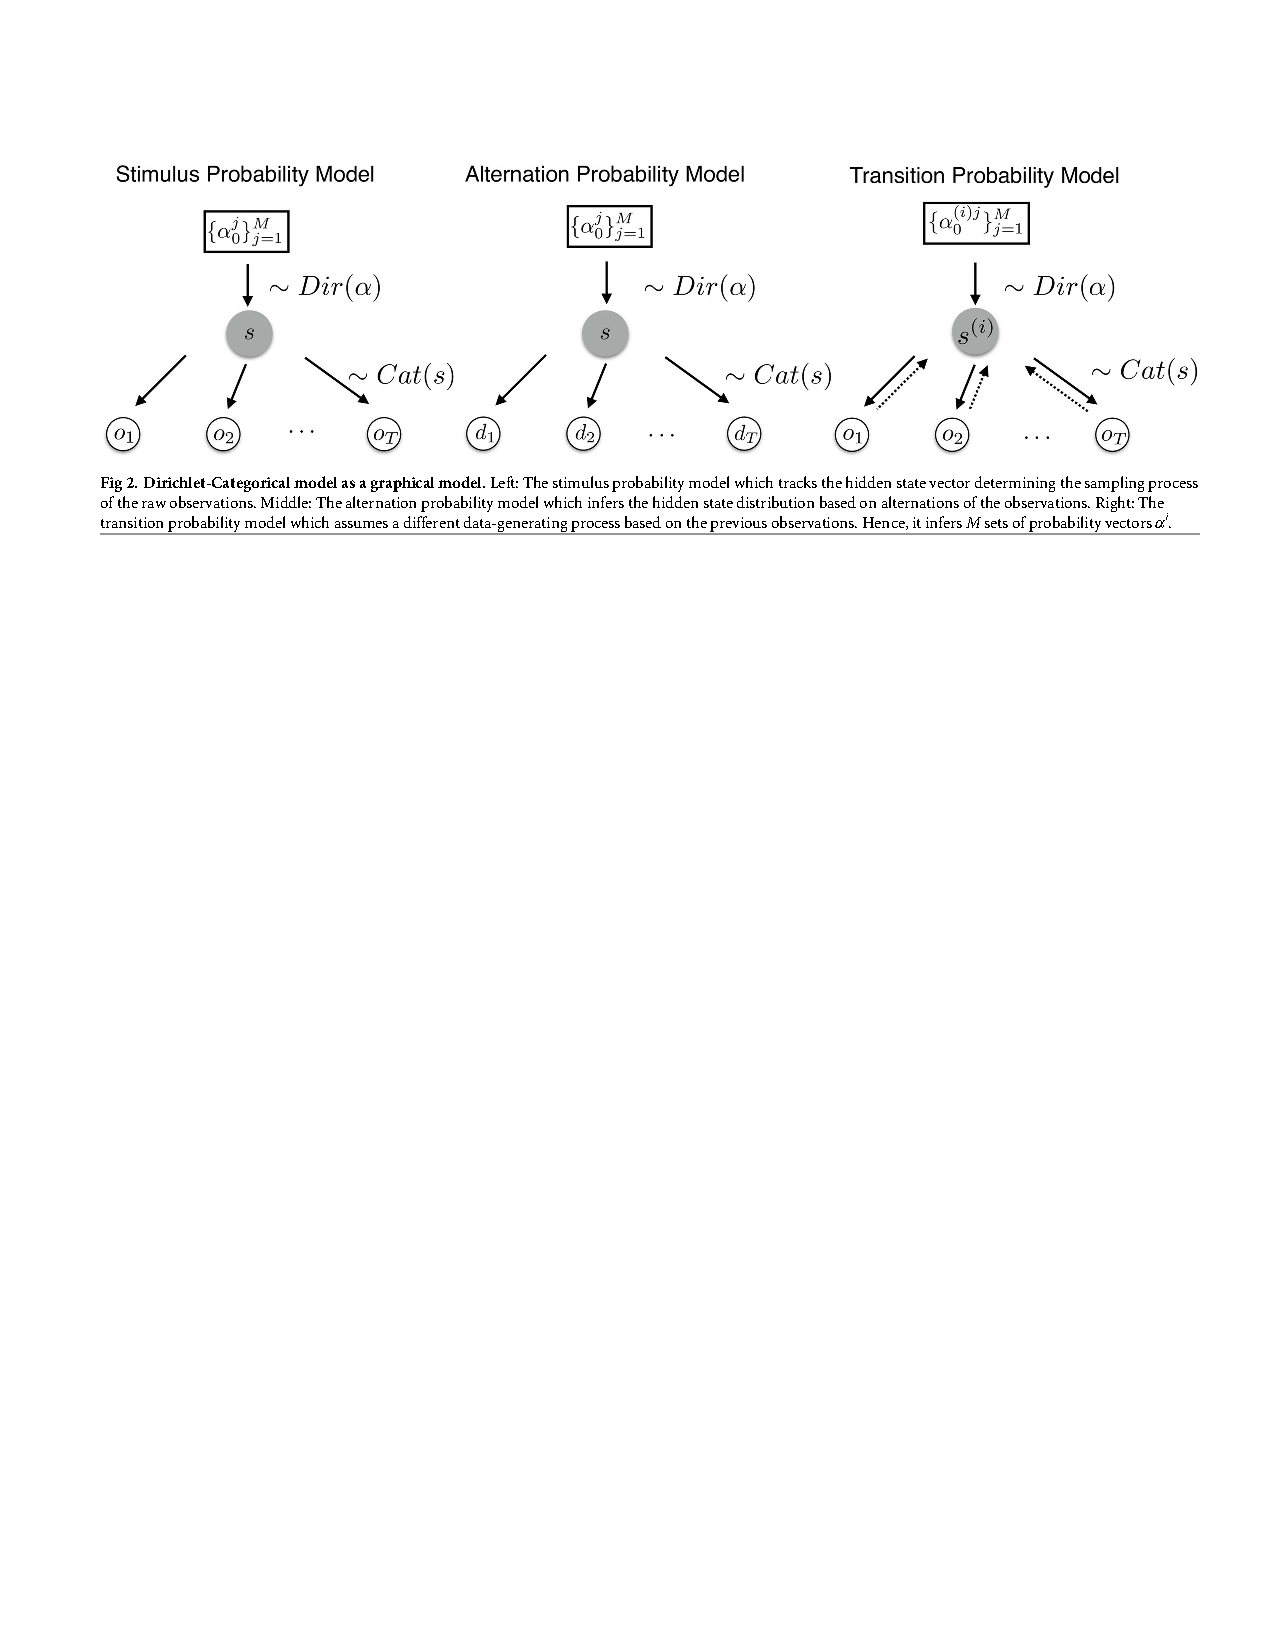
\includegraphics[width=0.55\linewidth]{2_Abbildungen/pfm_2_gijsen_theorie} \end{center}

\textcolor{darkblue}{Datenvorhersage} \vspace{-2mm}

\begin{center}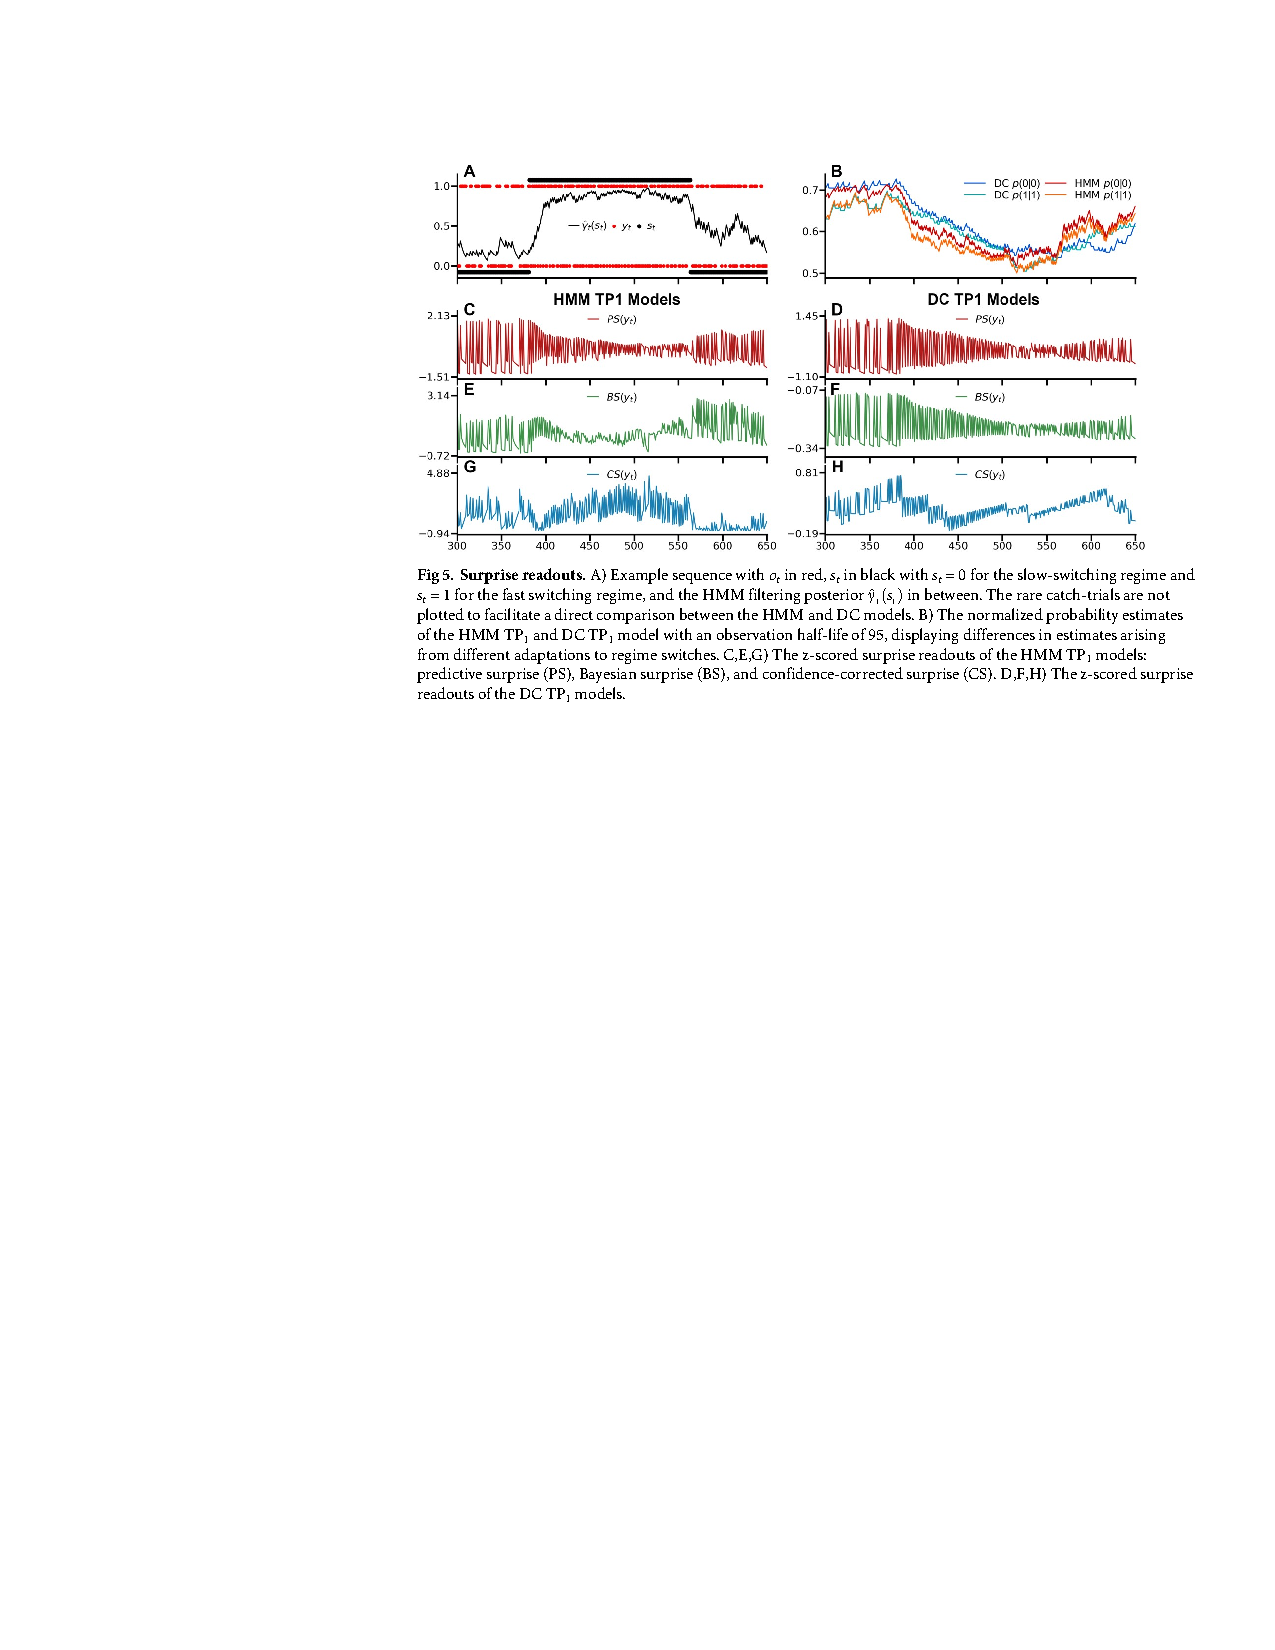
\includegraphics[width=0.55\linewidth]{2_Abbildungen/pfm_2_gijsen_datenvorhersage} \end{center}

\flushright
\footnotesize

Gijsen et al. (2021)
\end{frame}

\begin{frame}{Entwicklung mechanistischer neuropsychologischer Modelle}
\protect\hypertarget{entwicklung-mechanistischer-neuropsychologischer-modelle-5}{}
\textcolor{darkblue}{Datenanalyse} \vspace{2mm}

\begin{center}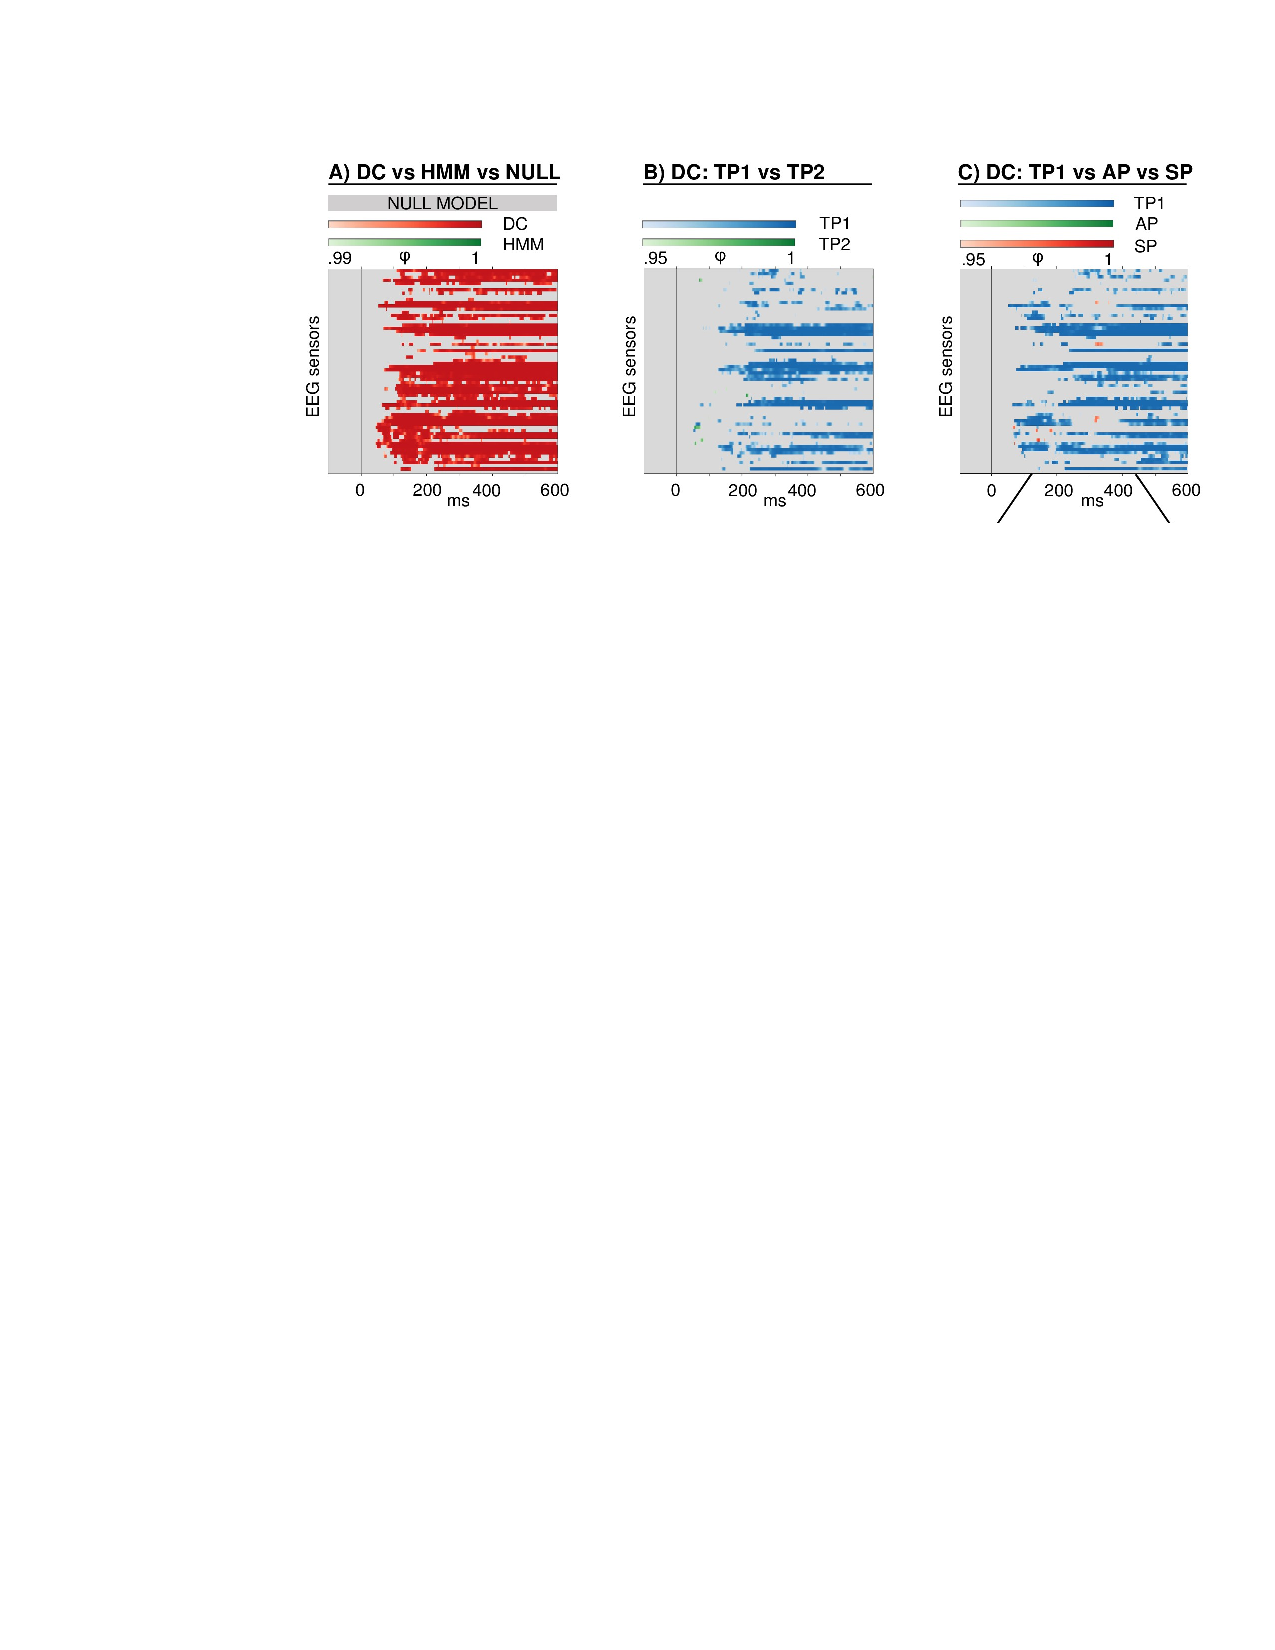
\includegraphics[width=0.9\linewidth]{2_Abbildungen/pfm_2_gijsen_datenanalyse_1} \end{center}

\begin{center}
\includegraphics[width=0.9\linewidth]{2_Abbildungen/pfm_2_gijsen_datenanalyse_2} \end{center}
\flushright
\footnotesize

Gijsen et al. (2021)
\end{frame}

\begin{frame}{}
\protect\hypertarget{section-5}{}
\setstretch{3}
\large

Einführung

Beispiele grundlagenorientierter psychologischer Forschung

\textbf{Beispiele anwendungsorientierter psychologischer Forschung}

Selbstkontrollfragen
\end{frame}

\begin{frame}{Behandlung psychiatrischer Erkrankungen}
\protect\hypertarget{behandlung-psychiatrischer-erkrankungen}{}
\begin{center}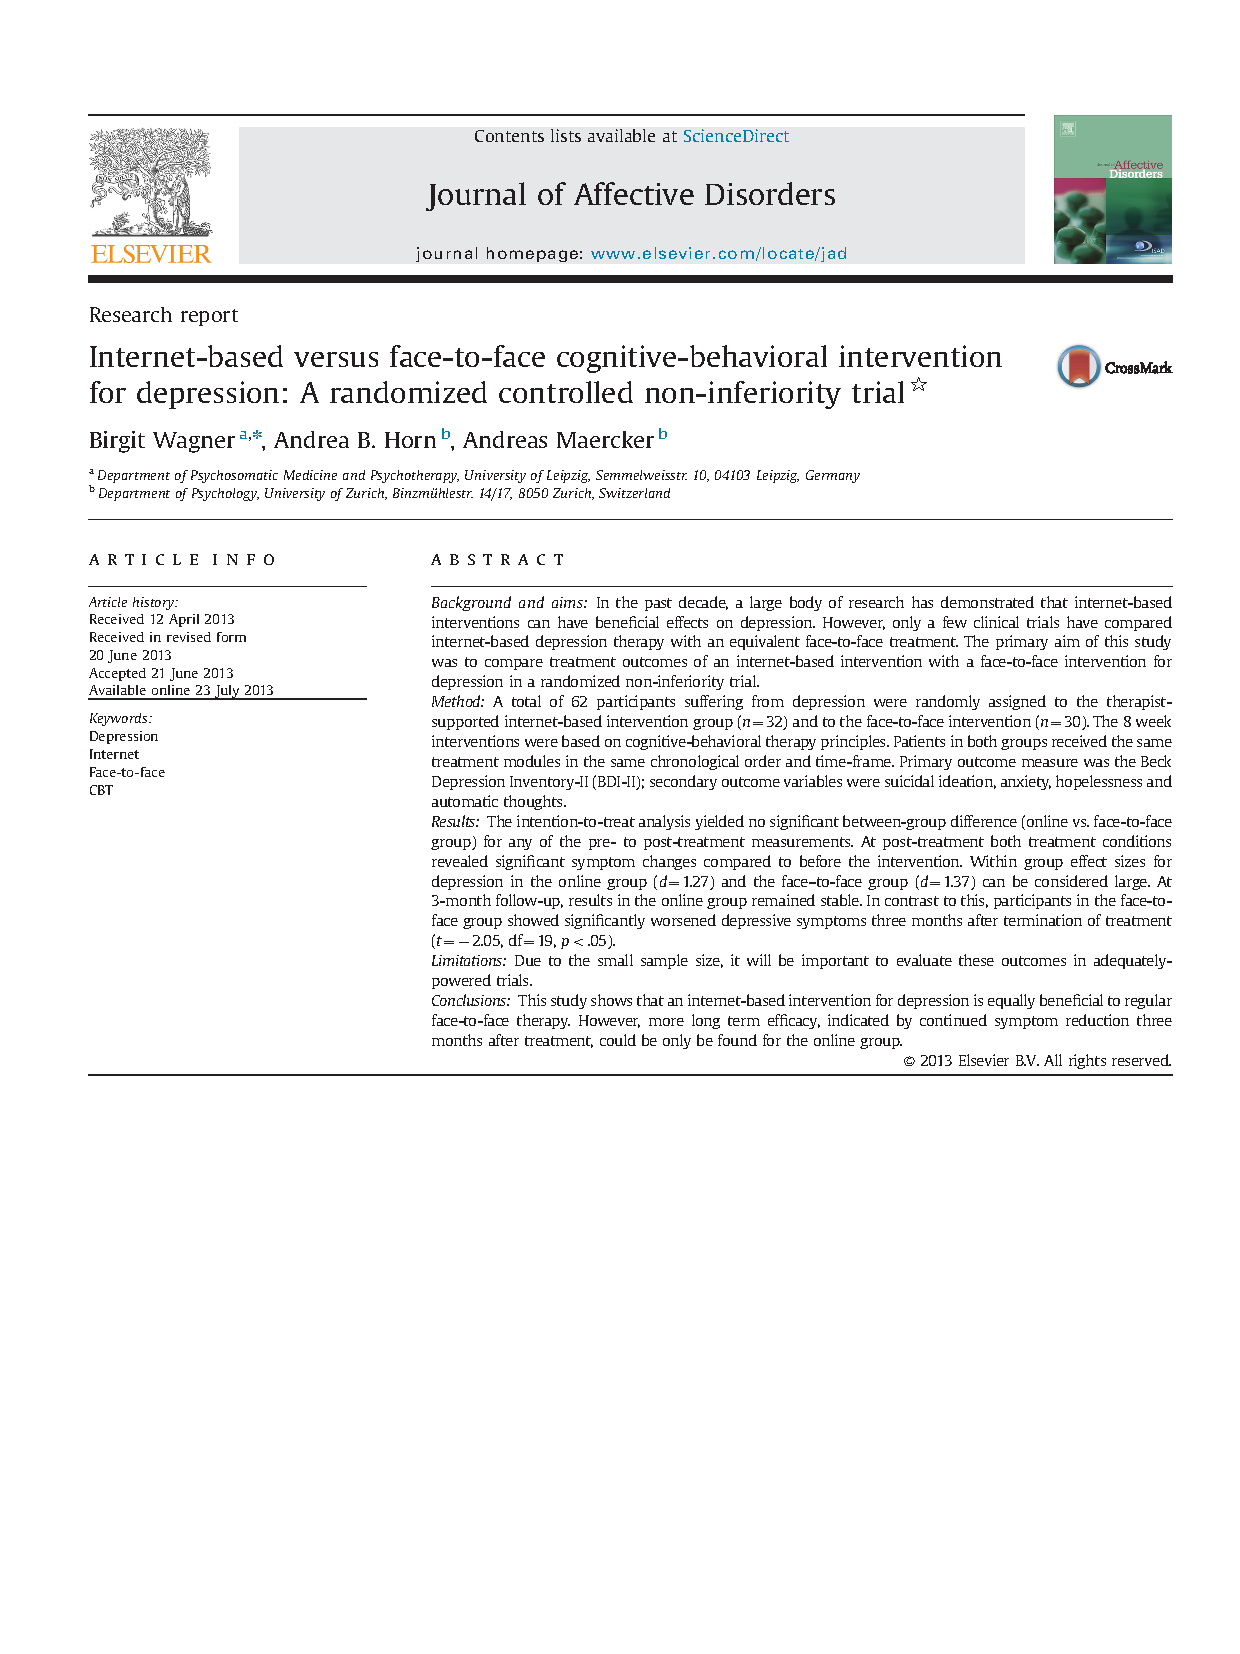
\includegraphics[width=0.6\linewidth]{2_Abbildungen/pfm_2_wagner_abstract} \end{center}

\flushright
\footnotesize

Wagner, Horn, and Maercker (2014)
\end{frame}

\begin{frame}{Behandlung psychiatrischer Erkrankungen}
\protect\hypertarget{behandlung-psychiatrischer-erkrankungen-1}{}
\textcolor{darkblue}{Evidenzbasierte Evaluation von Psychotherapieformen bei Depression}

\normalsize

Welche Therapieform ist bei Depression wirksamer?

\begin{center}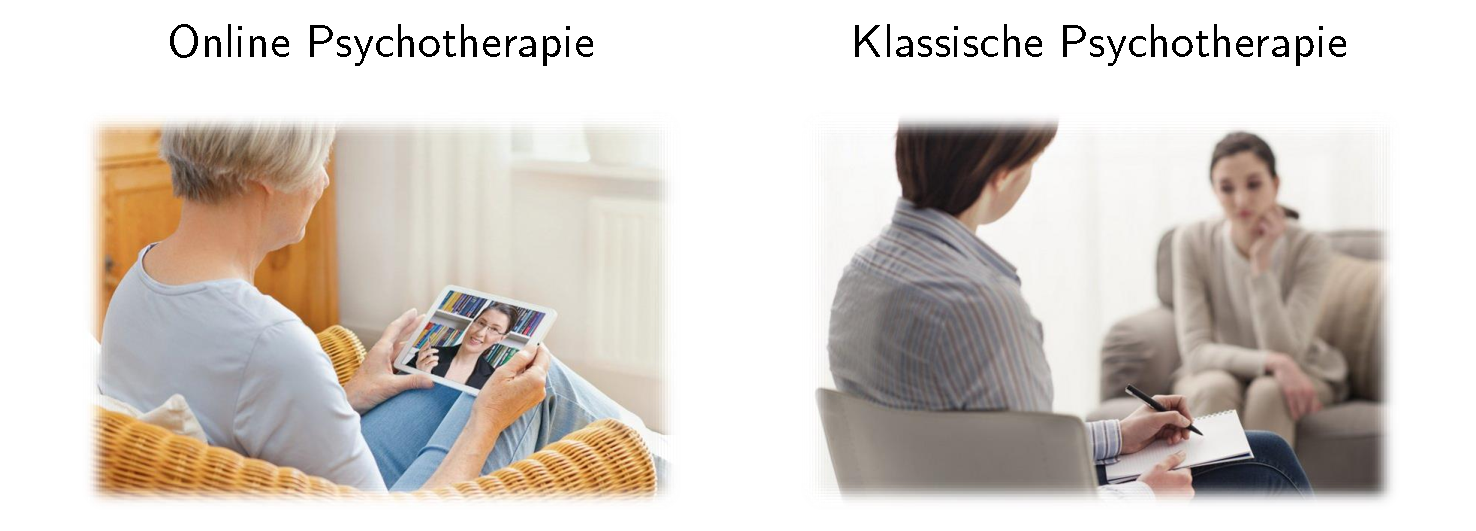
\includegraphics[width=1.1\linewidth]{2_Abbildungen/pfm_2_klinische_forschung} \end{center}
\end{frame}

\begin{frame}{Behandlung psychiatrischer Erkrankungen}
\protect\hypertarget{behandlung-psychiatrischer-erkrankungen-2}{}
\textcolor{darkblue}{Evidenzbasierte Evaluation von Psychotherapieformen bei Depression}

\normalsize

Becks Depressions-Inventar (BDI) zur Depressionsdiagnostik

\begin{center}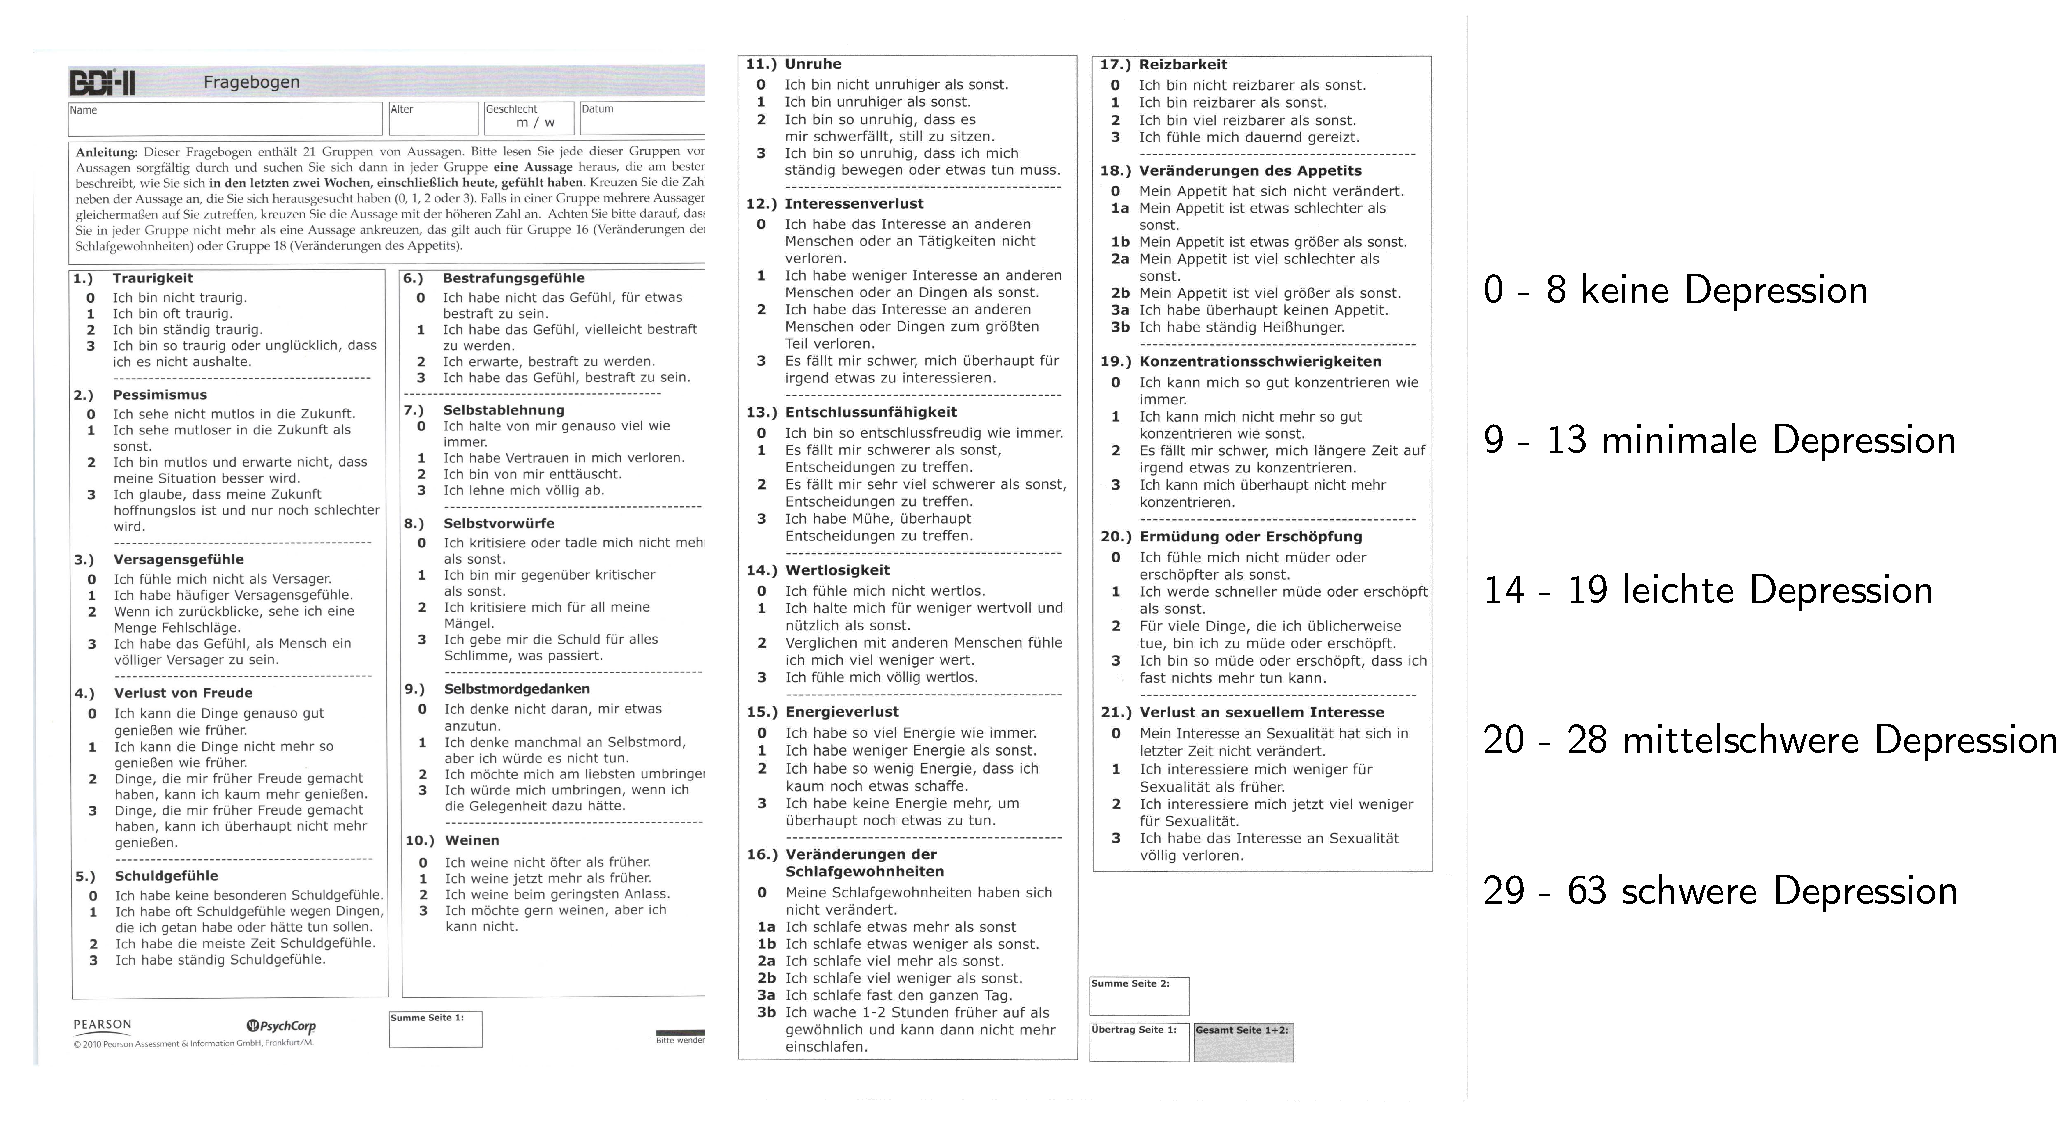
\includegraphics[width=1\linewidth]{2_Abbildungen/pfm_2_bdi} \end{center}
\end{frame}

\begin{frame}{Behandlung psychiatrischer Erkrankungen}
\protect\hypertarget{behandlung-psychiatrischer-erkrankungen-3}{}
\textcolor{darkblue}{Experimentelle Simulation} \setstretch{2} \small

\begin{itemize}
\tightlist
\item
  Zufällige Zuordnung mittelschwer Depressionserkrankter zu Online
  vs.~Klassisch
\item
  Im Wesentlichen identisches Behandlungsprotokoll in beiden Gruppen

  \begin{itemize}
  \tightlist
  \item
    \small 8 Wochen Kognitive Verhaltenstherapie nach Hautzinger (2021).
  \item
    Im Online Kontext nur schriftliches Feedback.
  \end{itemize}
\end{itemize}

\normalsize

\textcolor{darkblue}{Theorie} \small

\begin{itemize}
\tightlist
\item
  Es gibt Evidenz das internet-basierte Interventionen effektiv sind.
\item
  Es gibt Evidenz das Therapeuten-geleitete effektiver als
  selbstgeleitete Interventionen sind.
\end{itemize}

\normalsize

\textcolor{darkblue}{Datenvorhersage}

\small

\begin{itemize}
\tightlist
\item
  Die BDI-Differenzen zwischen Prä- und Posttherapie unterscheiden sich
  nicht.
\end{itemize}

\flushright
\footnotesize

Wagner, Horn, and Maercker (2014)
\end{frame}

\begin{frame}{Behandlung psychiatrischer Erkrankungen}
\protect\hypertarget{behandlung-psychiatrischer-erkrankungen-4}{}
\textcolor{darkblue}{Datenanalyse}

\begin{center}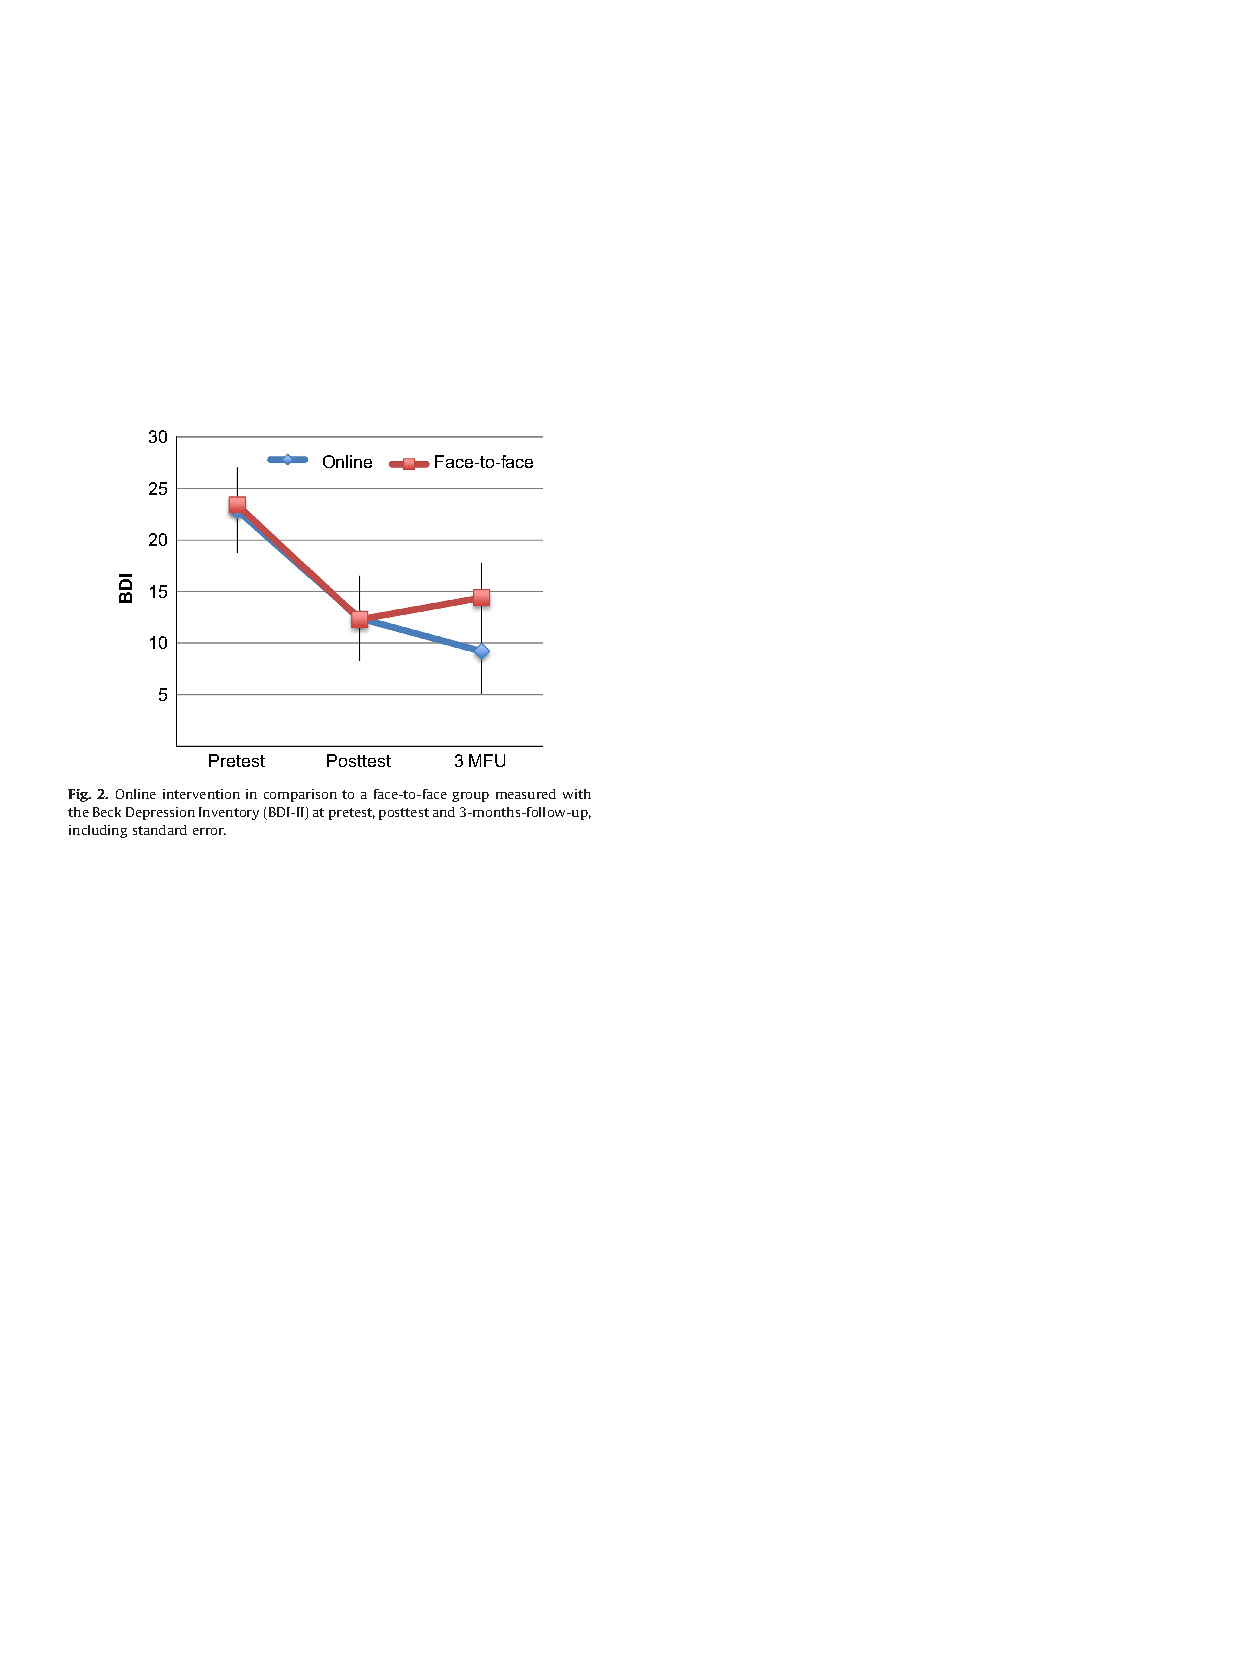
\includegraphics[width=0.75\linewidth]{2_Abbildungen/pfm_2_wagner_datenanalyse} \end{center}
\flushright
\footnotesize

Wagner, Horn, and Maercker (2014)
\end{frame}

\begin{frame}{Prognose zukünftigen Verhaltens und Handelns durch Big
Tech}
\protect\hypertarget{prognose-zukuxfcnftigen-verhaltens-und-handelns-durch-big-tech}{}
\vfill

\textcolor{darkblue}{Persönlichkeitspsychologie} \vspace{2mm}

\begin{center}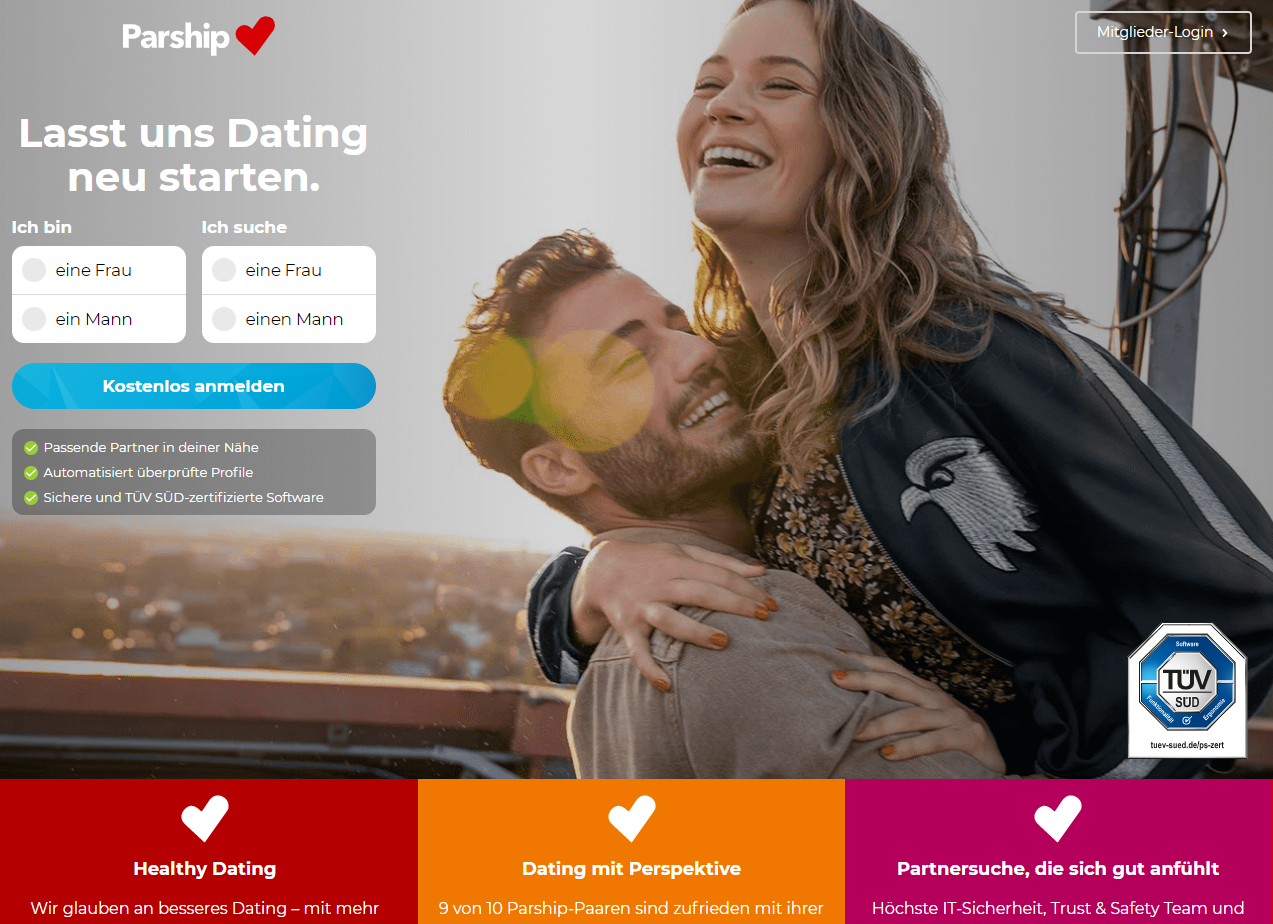
\includegraphics[width=0.75\linewidth]{2_Abbildungen/pfm_2_bigtech_parship} \end{center}
\vfill
\end{frame}

\begin{frame}{Prognose zukünftigen Verhaltens und Handelns durch Big
Tech}
\protect\hypertarget{prognose-zukuxfcnftigen-verhaltens-und-handelns-durch-big-tech-1}{}
\vfill

\textcolor{darkblue}{Emotionsforschung}

\begin{center}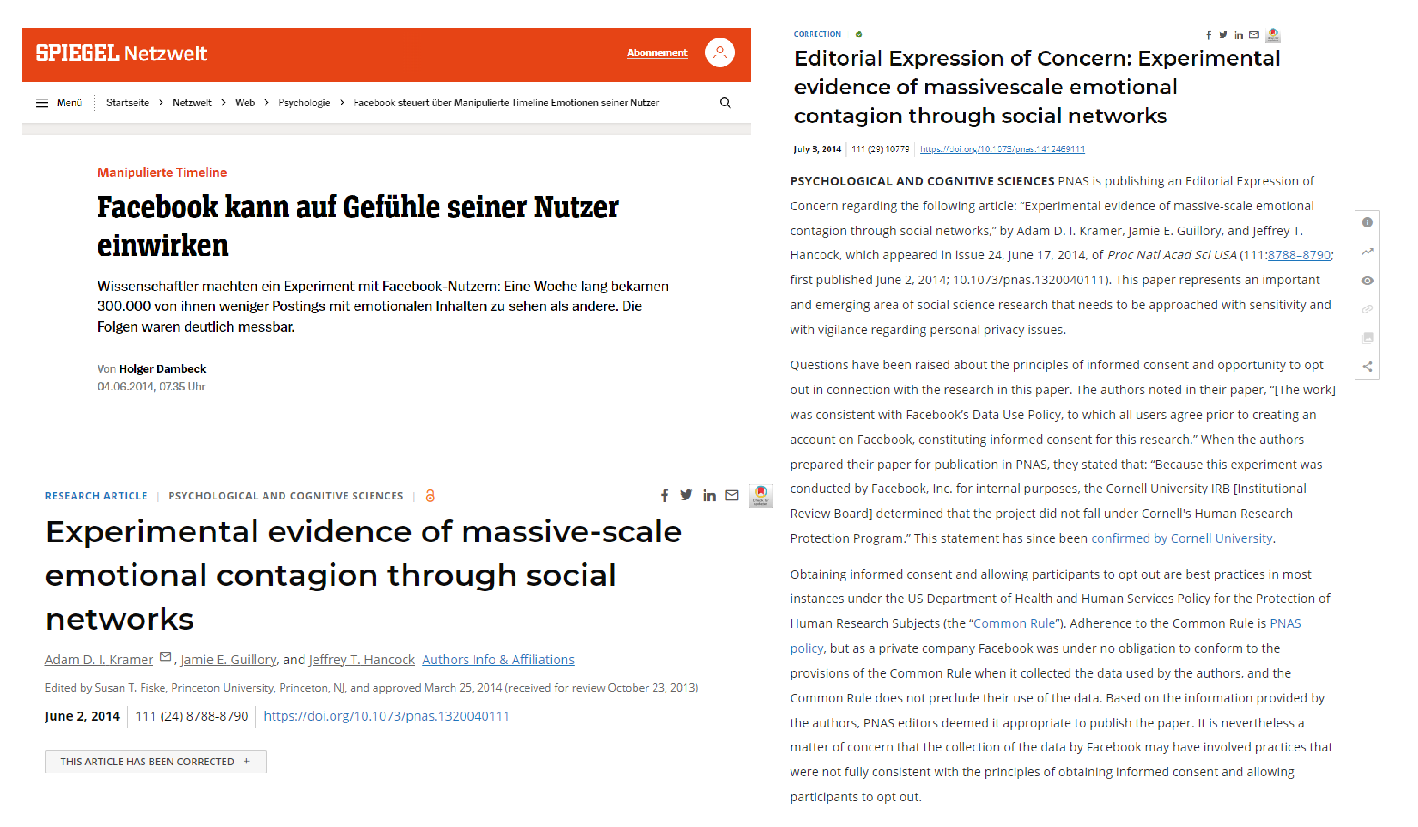
\includegraphics[width=1\linewidth]{2_Abbildungen/pfm_2_bigtech_facebook_experiment} \end{center}
\vfill
\end{frame}

\begin{frame}{Prognose zukünftigen Verhaltens und Handelns durch Big
Tech}
\protect\hypertarget{prognose-zukuxfcnftigen-verhaltens-und-handelns-durch-big-tech-2}{}
\vfill

\textcolor{darkblue}{Selbstkonzeptforschung}

\begin{center}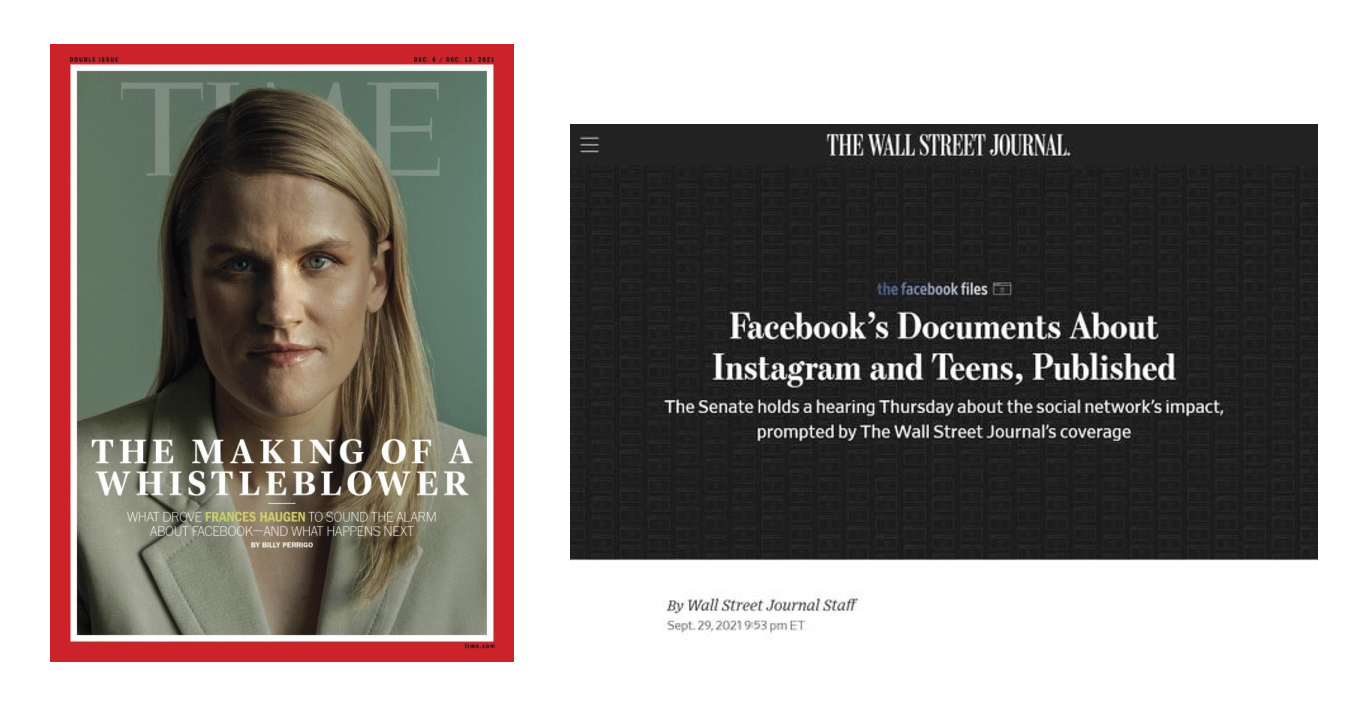
\includegraphics[width=1\linewidth]{2_Abbildungen/pfm_2_bigtech_facebook_files} \end{center}
\vfill
\end{frame}

\begin{frame}{Prognose zukünftigen Verhaltens und Handelns durch Big
Tech}
\protect\hypertarget{prognose-zukuxfcnftigen-verhaltens-und-handelns-durch-big-tech-3}{}
\vfill

\textcolor{darkblue}{Kaufentscheidungsverhalten}

\begin{center}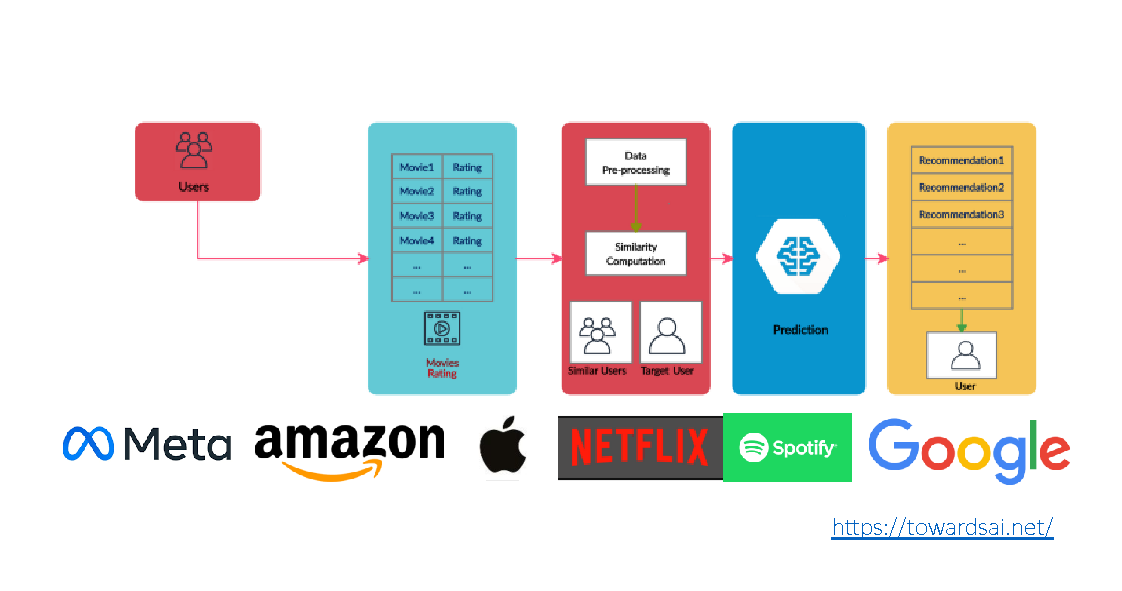
\includegraphics[width=1\linewidth]{2_Abbildungen/pfm_2_bigtech_recommender_systems} \end{center}
\vfill
\end{frame}

\begin{frame}{Prognose zukünftigen Verhaltens und Handelns durch Big
Tech}
\protect\hypertarget{prognose-zukuxfcnftigen-verhaltens-und-handelns-durch-big-tech-4}{}
\vfill

\textcolor{darkblue}{Sozialverhalten}

\begin{center}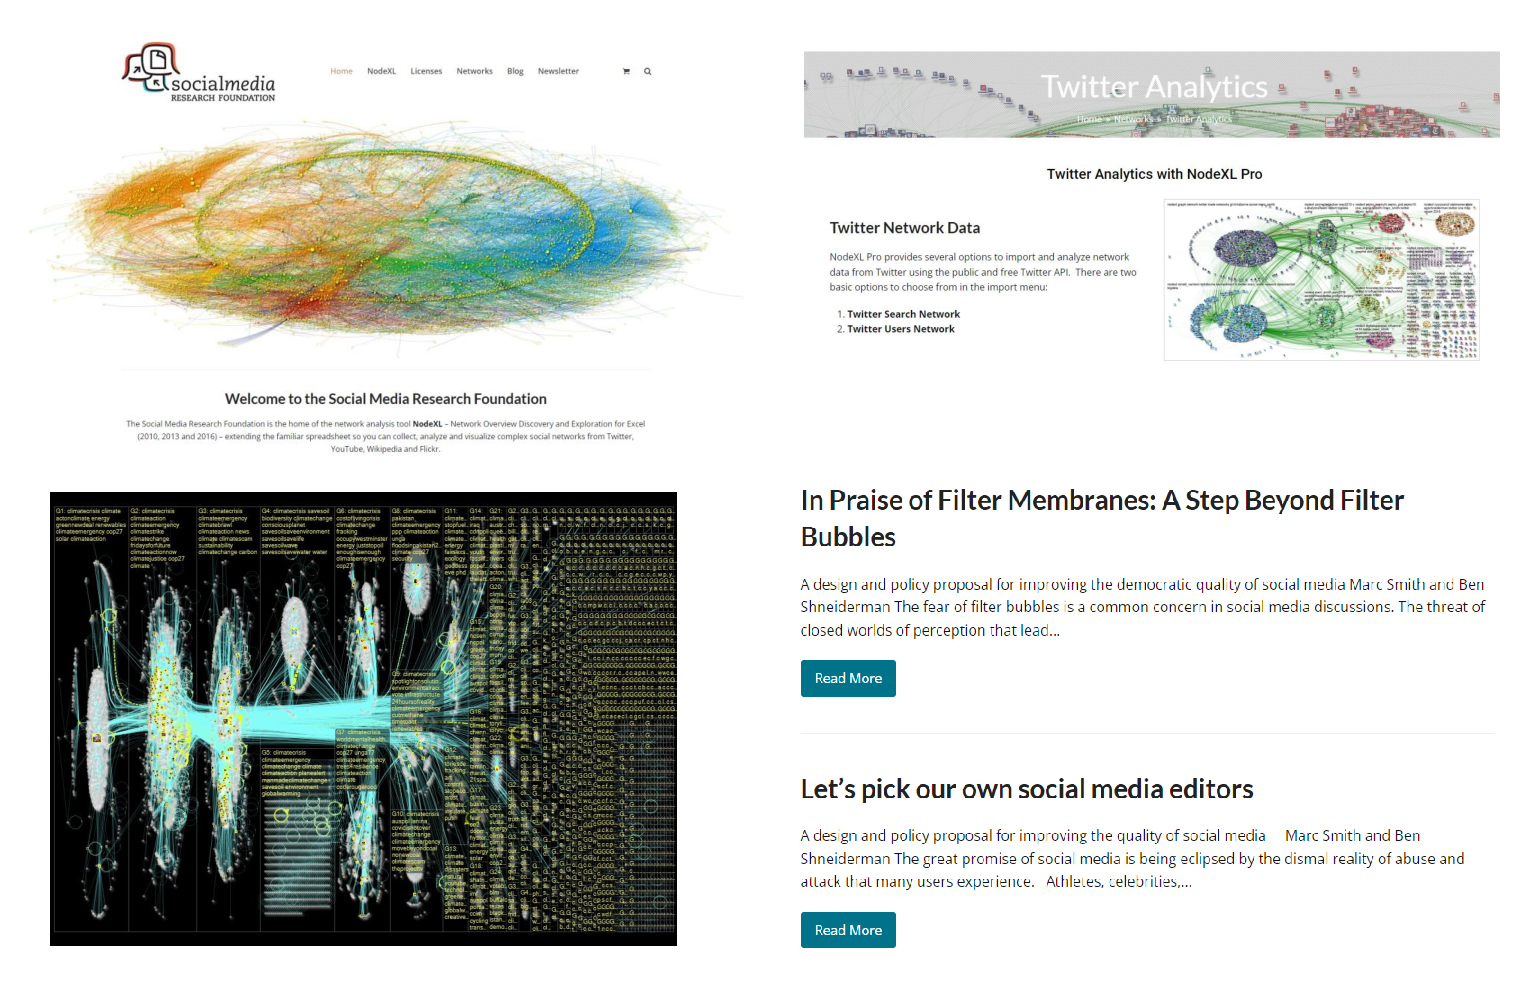
\includegraphics[width=0.9\linewidth]{2_Abbildungen/pfm_2_bigtech_sozialpsychologie} \end{center}
\vfill
\end{frame}

\begin{frame}{}
\protect\hypertarget{section-6}{}
\setstretch{3}
\large

Einführung

Beispiele grundlagenorientierter psychologischer Forschung

Beispiele anwendungsorientierter psychologischer Forschung

\textbf{Selbstkontrollfragen}
\end{frame}

\begin{frame}{Selbskontrollfragen}
\protect\hypertarget{selbskontrollfragen}{}
\small
\setstretch{3}

\begin{enumerate}
\tightlist
\item
  Definieren Sie den Begriff Psychologie.
\item
  Nennen Sie vier Aspekte psychologischer Wissenschaft.
\item
  Erläutern Sie den Begriff der psychologischen Grundlagenforschung.
\item
  Erläutern Sie den Begriff der anwendungsorientierten psychologischen
  Wissenschaft.
\end{enumerate}
\end{frame}

\begin{frame}{Referenzen}
\protect\hypertarget{referenzen}{}
\footnotesize

\hypertarget{refs}{}
\begin{CSLReferences}{1}{0}
\leavevmode\vadjust pre{\hypertarget{ref-friston_2005}{}}%
Friston, K. 2005. {``A Theory of Cortical Responses.''}
\emph{Philosophical Transactions of the Royal Society B: Biological
Sciences} 360 (1456): 815--36.
\url{https://doi.org/10.1098/rstb.2005.1622}.

\leavevmode\vadjust pre{\hypertarget{ref-gijsen_2021}{}}%
Gijsen, Sam, Miro Grundei, Robert T. Lange, Dirk Ostwald, and Felix
Blankenburg. 2021. {``Neural Surprise in Somatosensory {Bayesian}
Learning.''} Edited by Philipp Schwartenbeck. \emph{PLOS Computational
Biology} 17 (2): e1008068.
\url{https://doi.org/10.1371/journal.pcbi.1008068}.

\leavevmode\vadjust pre{\hypertarget{ref-hautzinger_2021}{}}%
Hautzinger, M. 2021. \emph{Kognitive {Verhaltenstherapie} Bei
{Depressionen}}. Beltz.

\leavevmode\vadjust pre{\hypertarget{ref-helmholtz_1867}{}}%
Helmholtz, Hermann von. 1867. \emph{Handbuch Der {Physiologischen}
{Optik}}. Leipzig: Voss.

\leavevmode\vadjust pre{\hypertarget{ref-horvath_2021}{}}%
Horvath, Lilla, Stanley Colcombe, Michael Milham, Shruti Ray, Philipp
Schwartenbeck, and Dirk Ostwald. 2021. {``Human {Belief} {State}-{Based}
{Exploration} and {Exploitation} in an {Information}-{Selective}
{Symmetric} {Reversal} {Bandit} {Task}.''} \emph{Computational Brain \&
Behavior} 4 (4): 442--62.
\url{https://doi.org/10.1007/s42113-021-00112-3}.

\leavevmode\vadjust pre{\hypertarget{ref-ostwald_2012}{}}%
Ostwald, Dirk, Bernhard Spitzer, Matthias Guggenmos, Timo T. Schmidt,
Stefan J. Kiebel, and Felix Blankenburg. 2012. {``Evidence for Neural
Encoding of {Bayesian} Surprise in Human Somatosensation.''}
\emph{NeuroImage} 62 (1): 177--88.
\url{https://doi.org/10.1016/j.neuroimage.2012.04.050}.

\leavevmode\vadjust pre{\hypertarget{ref-wagner_2014}{}}%
Wagner, Birgit, Andrea B. Horn, and Andreas Maercker. 2014.
{``Internet-Based Versus Face-to-Face Cognitive-Behavioral Intervention
for Depression: {A} Randomized Controlled Non-Inferiority Trial.''}
\emph{Journal of Affective Disorders} 152-154 (January): 113--21.
\url{https://doi.org/10.1016/j.jad.2013.06.032}.

\end{CSLReferences}
\end{frame}

\end{document}
